% !TeX encoding = UTF-8
% !TeX program = pdflatex
% !TeX spellcheck = it_IT

\documentclass[Lau, italian, noexaminfo]{sapthesis}

\usepackage[italian]{babel}
\usepackage[utf8]{inputenc}
\usepackage{hyperref}
\usepackage[chapter]{minted}
\usepackage{afterpage}
\usepackage{wrapfig}
\usepackage{csquotes} % Richiesto da biblatex.
\usepackage[style=numeric]{biblatex}

% Configurazione biblatex.
\addbibresource{references.bib}

% Configurazione di minted.
\definecolor{LightGray}{gray}{0.9}
\renewcommand{\listingscaption}{Codice sorgente}
\renewcommand{\listoflistingscaption}{Elenco dei codici sorgente}
\setminted{
    linenos=true,
    autogobble,
    breaklines,
}
% Per codici sorgente molto lunghi: meglio spezzarli su più pagine.
\newenvironment{longlisting}{\captionsetup{type=listing}}{}

% Definisco una sola volta alcuni test perché li riuso più volte.
\newcommand{\thetitle}{Progettazione e sviluppo delle API in linguaggio Go per il sistema di messaggistica domain-specific di SeismoCloud}
\newcommand{\theauthor}{Emanuele Petriglia}

% Configurazione di hyperref.
\hypersetup{
  pdftitle     = {\thetitle},
  pdfauthor    = {\theauthor},
  colorlinks   = true,
  urlcolor     = black,
  linkcolor    = black,
  citecolor    = black
}

% Configurazione di sapthesis.
\title{\thetitle}
\author{\theauthor}
\IDnumber{1798177}
\course{Informatica}
\courseorganizer{Facoltà di Ingegneria dell'informazione, informatica e statistica}
\AcademicYear{2020/2021}
\copyyear{2021}
\advisor{Prof. Emanuele Panizzi}

\authoremail{petriglia.1798177@studenti.uniroma1.it}
\versiondate{28 luglio 2021}
\copyrightstatement{© 2021 Emanuele Petriglia. Tutti i diritti riservati. Rilasciata con licenza Creative Commons Attribuzione - Condividi allo stesso modo 4.0 Internazionale (CC BY-SA 4.0).}

\begin{document}

\frontmatter

\maketitle

\begin{abstract}

L'oggetto della relazione di tirocinio è lo studio, progettazione e implementazione di API per costruire un servizio di messaggistica specifico per il progetto SeismoCloud.

La relazione è divisa in cinque capitoli: \hyperref[ch:intro]{un'\textbf{introduzione} (Capitolo \ref{ch:intro})} al progetto SeismoCloud e all'obiettivo del tirocinio, \hyperref[ch:analisi]{l'\textbf{analisi dei requisiti} (Capitolo \ref{ch:analisi})}, che descrive in maniera dettagliata la funzionalità progettata e sviluppata, la \hyperref[ch:progg]{\textbf{progettazione} (Capitolo \ref{ch:progg})} delle API e del database, \hyperref[ch:impl]{l'\textbf{implementazione} (Capitolo \ref{ch:impl})} della funzionalità, con le scelte e le sfide implementative incontrate, e le \hyperref[ch:concl]{\textbf{conclusioni} (Capitolo \ref{ch:concl})} che offrono spunti sulle possibili vie per proseguire il lavoro.

L'ultimo capitolo dei \hyperref[ch:ringr]{\textbf{ringraziamenti}} compare solo nella presente versione, redatta dopo la consegna ufficiale della relazione.

\end{abstract}

\tableofcontents

\mainmatter

\chapter{Introduzione}
\label{ch:intro}

\section{Il progetto SeismoCloud}

\begin{wrapfigure}{r}{0.25\textwidth}
\centering

\includegraphics[scale=0.15]{assets/01/logoseismocloud.png}
\caption{Logo di SeismoCloud.}
\label{fig:logo}
\end{wrapfigure}

SeismoCloud \cite{seismocloud}, il cui logo è mostrato nella figura \ref{fig:logo}, è un progetto rilevazione e segnalazione di terremoti basata su una rete di sismometri diffusi a livello nazionale. Il progetto nasce dalla collaborazione dell'Università degli Studi di Roma ``La Sapienza'' e l'Istituto Nazionale di Geofisica e Vulcanologia (INGV). Lo scopo del progetto è l'Earthquake Early Warning (EEW), che consiste nel controllo dell'attività sismica e, in caso di un terremoto, la notifica agli utenti interessati.

Poiché i sismometri previsti dal progetto sono a basso costo, sono imprecisi e pertanto solo con una grande quantità è possibile effettuare una stima affidabile del verificarsi di un terremoto. Per tale motivazione il sistema EEW non è attualmente abilitato. Ci sono più di un centinaio di sismometri attivi a livello nazionale, numero in crescita di anno in anno, ma, da come si evince dalla figura \ref{fig:distribuzione}, è necessario che siano ben distribuiti sul territorio.

Una funzionalità di SeismoCloud è la possibilità di formare dei gruppi di utenti, spesso organizzati dalle scuole, per condividere statistiche sui propri sismometri.
\begin{figure}[ht]
\centering
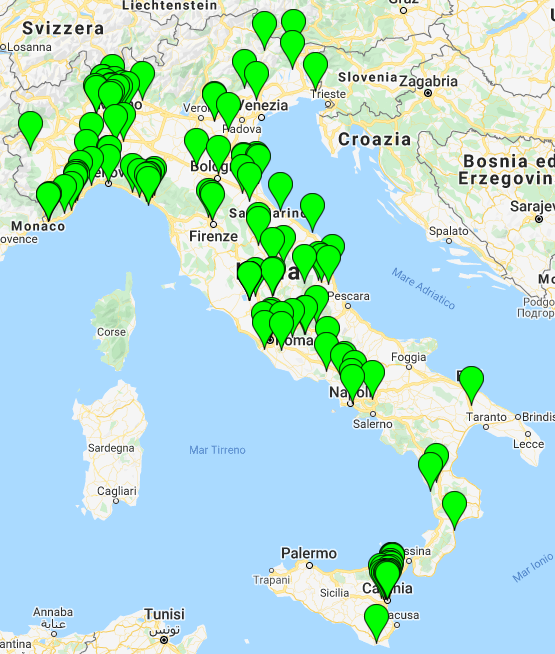
\includegraphics[scale=0.35]{assets/01/distribuzione_sismometri.png}
\caption{I sismometri attivi a livello nazionale.}
\label{fig:distribuzione}
\end{figure}

\paragraph{Tipologie di sismometri} I sismometri possono essere di due tipologie: una fissa costituita da dispositivi \textit{Internet of Things} (Arduino, NodeMCU e Raspberry PI) a basso costo e open source, che l'utente può costruire seguendo le istruzioni fornite sul sito web del progetto, oppure una mobile che consiste in un'applicazione per telefoni (Android e iOS).

L'applicazione mobile permette agli utenti di gestire e monitorare lo stato dei propri sismometri e della rete nazionale, in più rende il telefono esso stesso un sismometro, sfruttando l'accelerometro per rilevare le vibrazioni nei momenti in cui il telefono non viene utilizzato ed è poggiato su un supporto orizzontale.

Tutti i sismometri sono registrati all'interno del server di SeismoCloud. Ogni volta che uno di questi rileva una vibrazione, invia via Internet i dati al server, che tramite algoritmi dedicati, è in grado di capire se si tratta un terremoto nei primi secondi dall'inizio della scossa. Nella figura \ref{fig:rete} è possibile osservare il funzionamento della rete.

\begin{figure}[ht!]
\centering
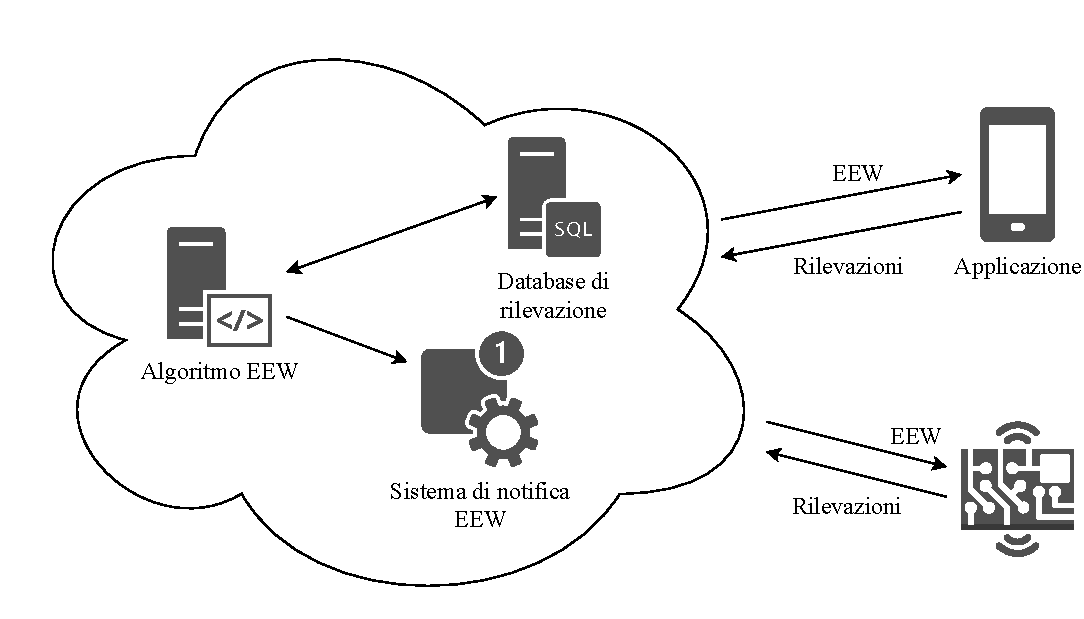
\includegraphics[width=\textwidth]{assets/01/rete.pdf}
\caption{Architettura della rete di SeismoCloud.}
\label{fig:rete}
\end{figure}

\section{Architettura server di SeismoCloud}

Prima di descrivere l'obiettivo del tirocinio, è utile tenere in mente l'architettura lato server di SeismoCloud, mostrata nella figura \ref{fig:architettura}. I vari client possono interagire con il server attraverso il protocollo HTTPS e MQTT su quattro componenti:

\begin{itemize}
\item \textbf{API firmware}: espone le API necessarie per aggiornare i sistemi dei sismometri fissi;
\item \textbf{Broker MQTT}: gestisce l'arrivo dei dati delle rilevazioni dei sismometri;
\item \textbf{API principali}: espone la maggior parte delle API di SeismoCloud;
\item \textbf{Keycloak}: espone il servizio di registrazione e autenticazione degli utenti.
\end{itemize}

Le API principali richiedono quasi tutte l'autenticazione, ciò viene garantito tramite l'utilizzo di \texttt{token} che il client invia in ogni richiesta e che il server può verificare. Keycloak eroga tali token ai client.

Nel sistema è presente MariaDB come database relazionale per la conservazione dei dati. Nello stesso database sono salvati sia le rilevazioni degli eventi sismici che tutti i dati relativi ai terremoti, ai gruppi, i sismometri e altro.

È presente anche un server di \textit{file storage} MinIO, in cui sono salvati i firmware da inviare ai sismometri fissi.

Il componente \textit{Worker} si occupa invece di lavori asincroni eseguiti in modo distaccato dall'interazione con i client, tra cui l'aggiornamento della lista dei terremoti nel database e l'invio delle notifiche ai client.

\begin{figure}[ht!]
\centering
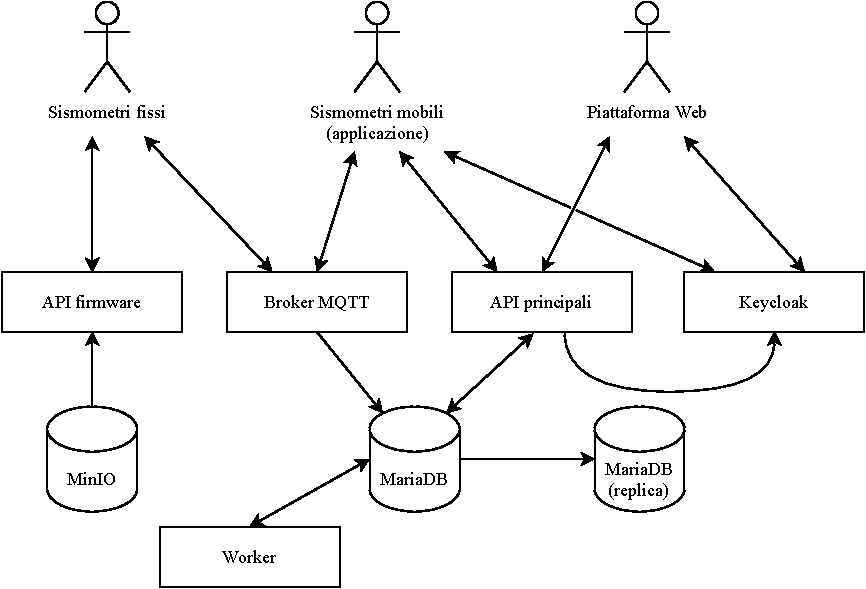
\includegraphics[width=\textwidth]{assets/01/architettura.pdf}
\caption{Architettura server di SeismoCloud.}
\label{fig:architettura}
\end{figure}

\section{Obiettivo del tirocinio}

L'obiettivo, svolto all'interno del team di sviluppo di SeismoCloud, consiste nella progettazione e nello sviluppo delle API per il servizio di messaggistica specifico per lo scambio di informazioni sui terremoti tra gli utenti. Tale funzionalità va a rafforzare lo scopo principale del progetto, cioè il servizio di EEW, in modo da aumentare, tramite l'interazione sociale, il bacino di utenti e quindi il numero di sismometri.

Il lavoro prosegue direttamente l'attività svolta dallo studente Michele Spina, che ha lavorato nello studio e progettazione dell'interfaccia utente per la funzionalità di messaggistica. Il suo lavoro è descritto in dettaglio nella relazione ``Design e development in Android dell’UI per l'interazione sociale in SeismoCloud'' \cite{michele}.

\chapter{Analisi dei requisiti}
\label{ch:analisi}

Prima di procedere nella progettazione è fondamentale analizzare il problema per poi costruire un modello che soddisfi i requisiti trovati. Per tale scopo prima vengono prima riportati i risultati del lavoro di Michele Spina, tra cui parte delle interfacce grafiche sviluppate, dopodiché si procede con la modellazione più approfondita e precisa.

\section{Origine della funzionalità}

La necessità di trovare uno spazio di interazione sociale, per lo scambio di informazioni relative alle scosse più recenti, è risultata da un lavoro di interviste del tirocinante Daniele Proietti. In seguito il tirocinante Michele Spina ha preso in carico i risultati per progettare più nel dettaglio la funzionalità, ponendo attenzione sulle interfacce utente per sistema operativo Android. L'attuale sistema di segnalazioni presente in SeismoCloud differisce dalla necessità scoperta in base ai soggetti di questi due sistemi: nel primo caso sono i sismometri che inviano le rilevazioni sismiche, nel secondo caso sono gli utenti che interagiscono tra di loro.

\paragraph{Perché le chat?} La scelta di utilizzare un approccio basato su chat deriva dell'estrema diffusione di sistemi di messaggistica, per cui l'utente non dovrebbe avere difficoltà a utilizzare questo nuovo sistema. C'è però una differenza sostanziale di fondo, poiché il nuovo sistema è focalizzato sul dominio di SeismoCloud, cioè i terremoti, mentre un sistema generale di messaggistica non ha uno scopo preciso. Questo fatto è importante per capire le decisioni prese nella modellazione delle funzionalità.

\paragraph{Elenco delle chat} L'utente può interagire con altri in delle chat pubbliche, dei luoghi in cui si possono inviare e ricevere dei messaggi di varia tipologia. La figura \ref{fig:android_menu} mostra la schermata principale da cui l'utente può selezionare la singola chat. L'elenco è ordinato dalla chat aggiornata più di recente. Nell'interfaccia si possono notare dettagli importanti tra cui: il nome della chat, legato al luogo nel quale sono state sentire le scosse, un'anteprima dell'ultimo messaggio, un contatore dei messaggi non letti e la data, o l'ora, dell'ultimo aggiornamento.

Si sottolinea che le chat sono pubbliche e accessibili sia in scrittura che in lettura per tutti gli utenti, in modo indifferente dalla loro posizione geografica. Il motivo è che un utente lontano dal sisma potrebbe voler chiedere informazioni su quanto accaduto.

\paragraph{I messaggi} Una volta selezionata la chat, l'utente, oltre a inviare un messaggio, può scorrere la cronologia dei messaggi inviati, come mostrato nella figura \ref{fig:android_chat}. Per ogni messaggio è indicato il nome del mittente, la località di invio del messaggio e l'ora di invio. Ci sono tre tipologie di messaggi previsti:

\begin{itemize}
\item Messaggi testuali, che contengono soltanto testo;
\item Messaggi fotografici, che consistono in una singola foto;
\item Messaggi \textit{slider}, che consistono in un valore numerico, rappresentato come slider, cioè una barra orizzontale composta da passi, ognuno dei quali rappresenta un valore, accompagnato da una formula testuale esplicativa che è prefissata.
\end{itemize}

Tra le tre tipologie quello unico e particolare, non presente in altri sistemi di messaggistica, è lo slider. Il valore viene fatto corrispondere alla scala macrosismica Mercalli-Cancani-Sieberg (MCS-1930) \cite{mcs}, con i primi tre valori accorpati perché rappresentano scosse talmente leggere da essere difficilmente rilevabili da un essere umano. La figura \ref{fig:android_slider} è un esempio di un messaggio slider con un valore corrispondente al quarto grado VI della scala.

Riguardo l'invio di un messaggio, la barra inferiore contiene i pulsanti necessari per inviare un messaggio per ogni tipo. Un messaggio può essere inviato opzionalmente con la posizione geografica approssimativa.

\paragraph{Creazione di una chat} Nella barra in alto della schermata principale è possibile premere un pulsante per avviare la creazione di una chat. Una chat è vincolata alla posiziona geografica dell'utente che la crea, per cui l'utente è obbligato a condividere la posizione geografica. La creazione di una chat non è libera, è il sistema a decidere se creare la chat basandosi sulla posizione e sulla data e ora della richiesta. Il nome delle chat è generato in automatico dal sistema, e appena viene creata diventa visibile nell'elenco solo dopo l'invio di un primo messaggio.

\begin{figure}[p]
\centering

% Trucco con minipage per posizionare due figure una accanto all'altra con le loro rispettive didascalie. Attenzione agli spazzi e ai ritorni a capo, non ci devono essere in mezzo altrimenti non funziona!
\begin{minipage}{0.45\linewidth}
\centering
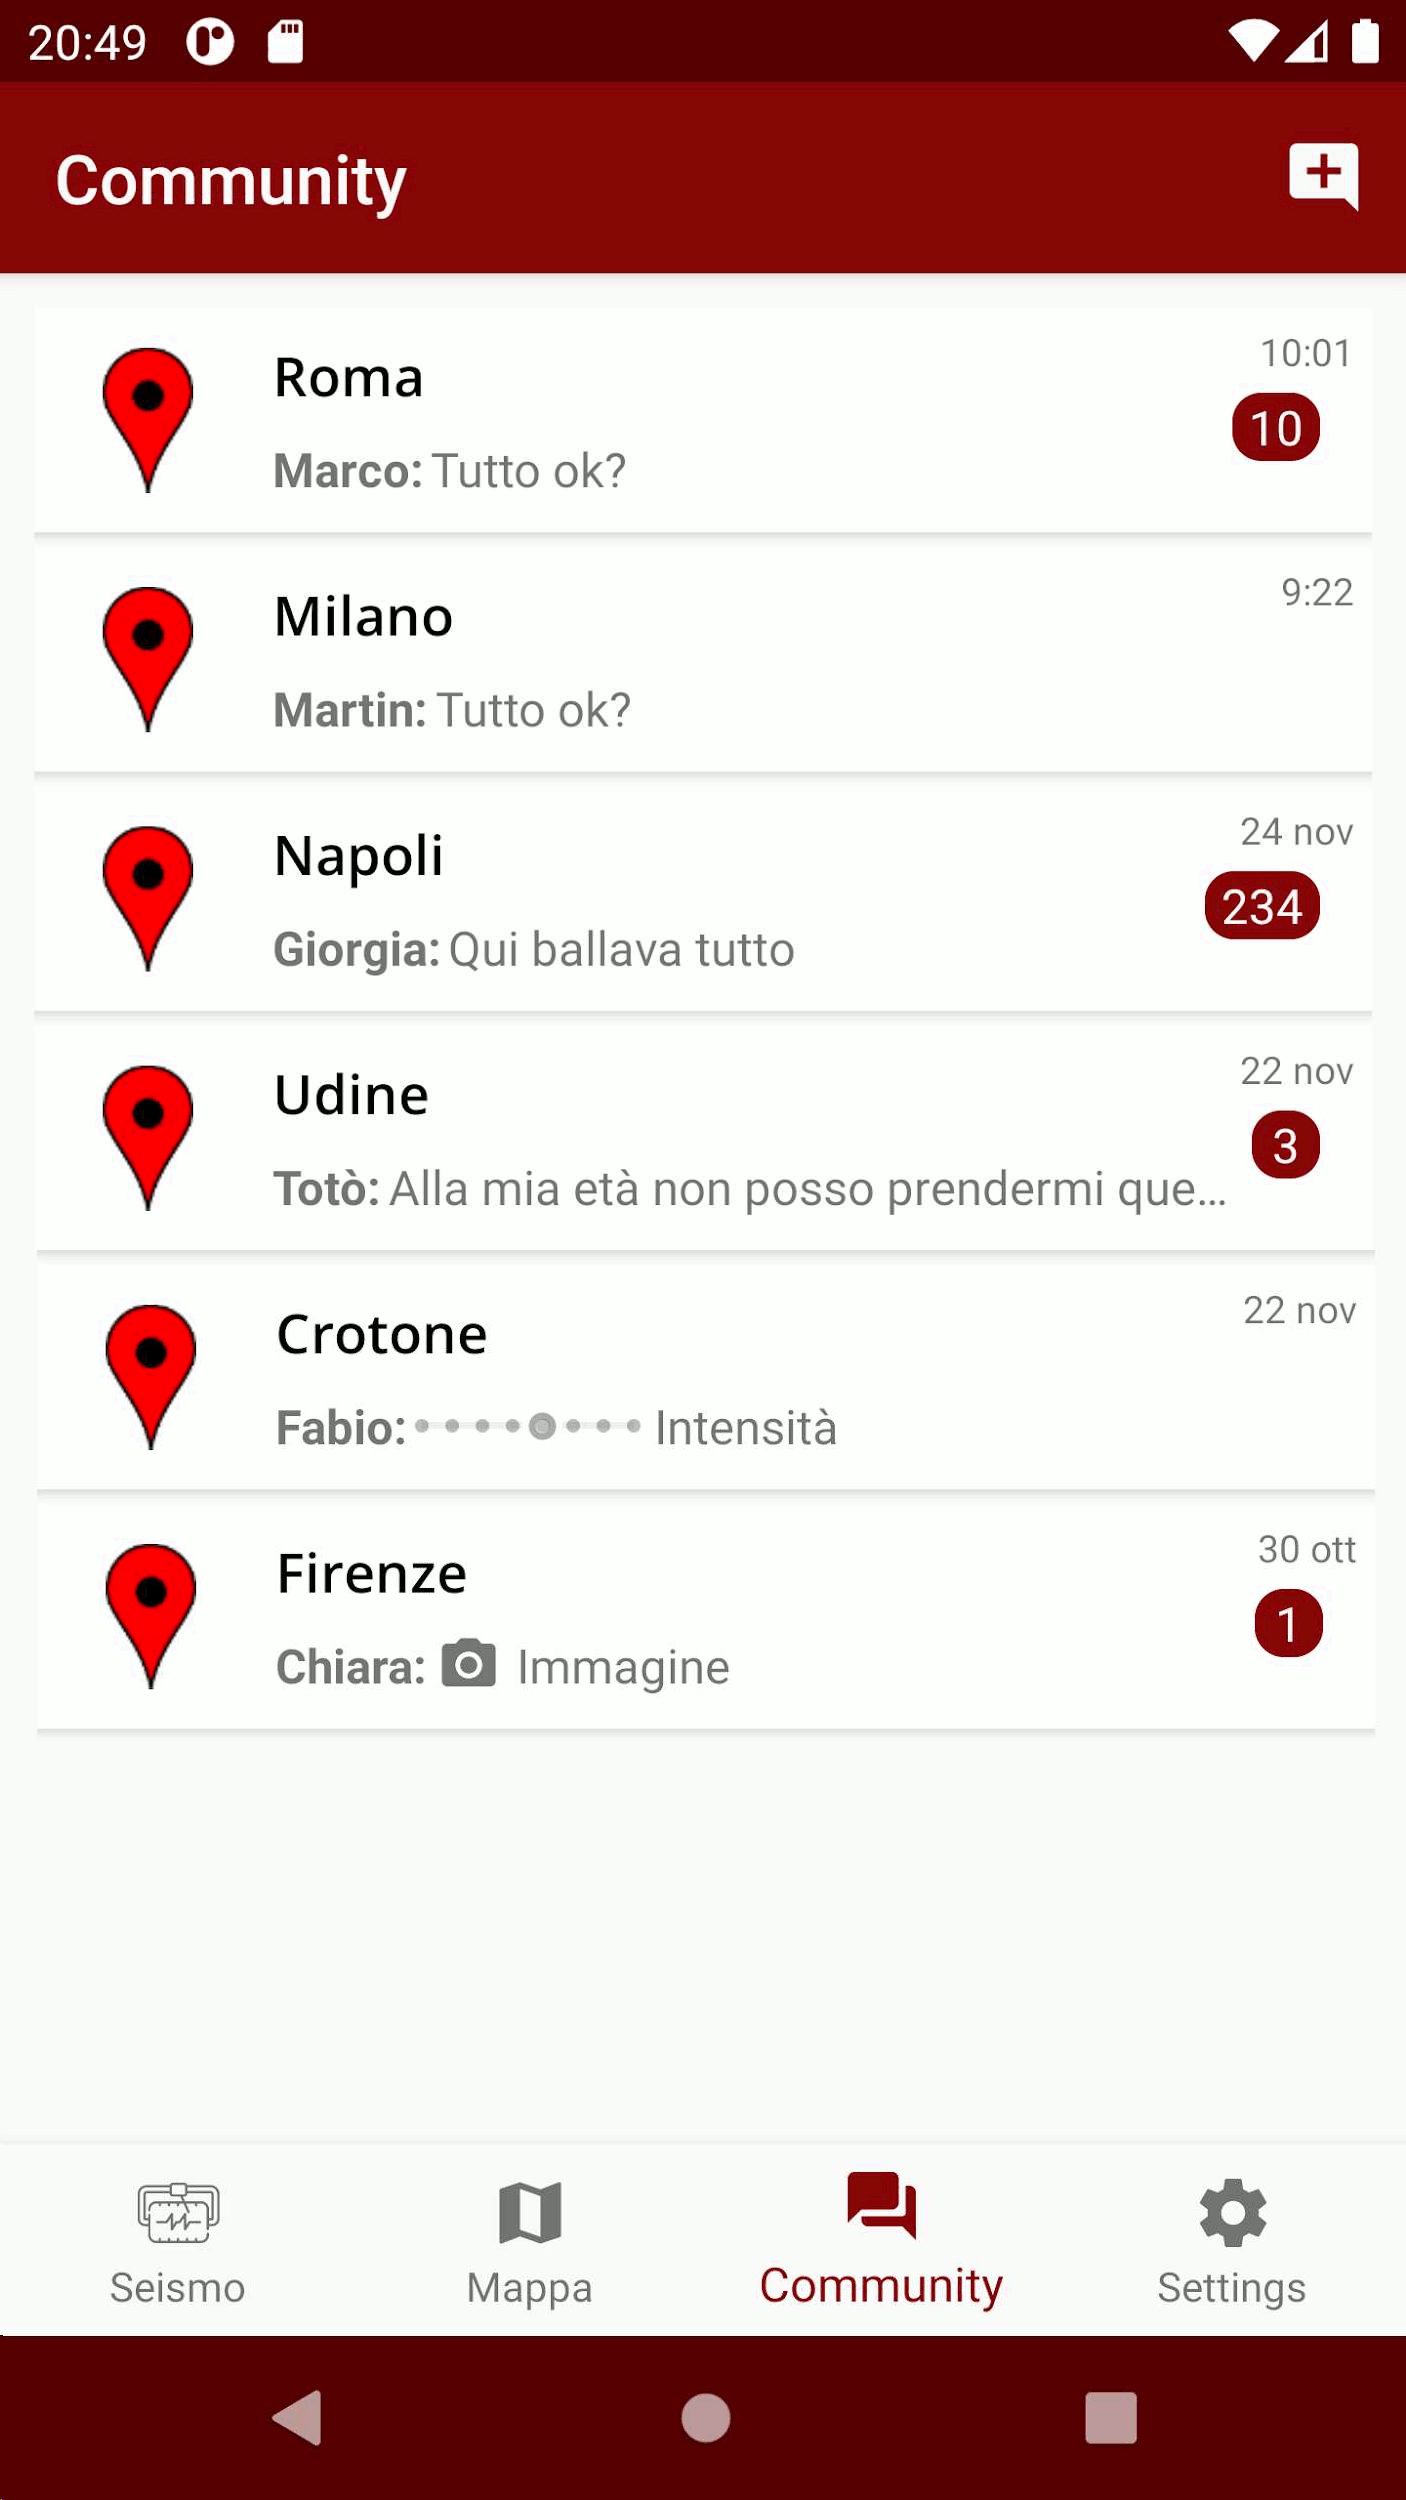
\includegraphics[width=0.85\linewidth]{assets/02/menu.png}
\caption{Schermata con l'elenco delle chat.}
\label{fig:android_menu}
\end{minipage}\hfill
\begin{minipage}{0.45\linewidth}
\centering
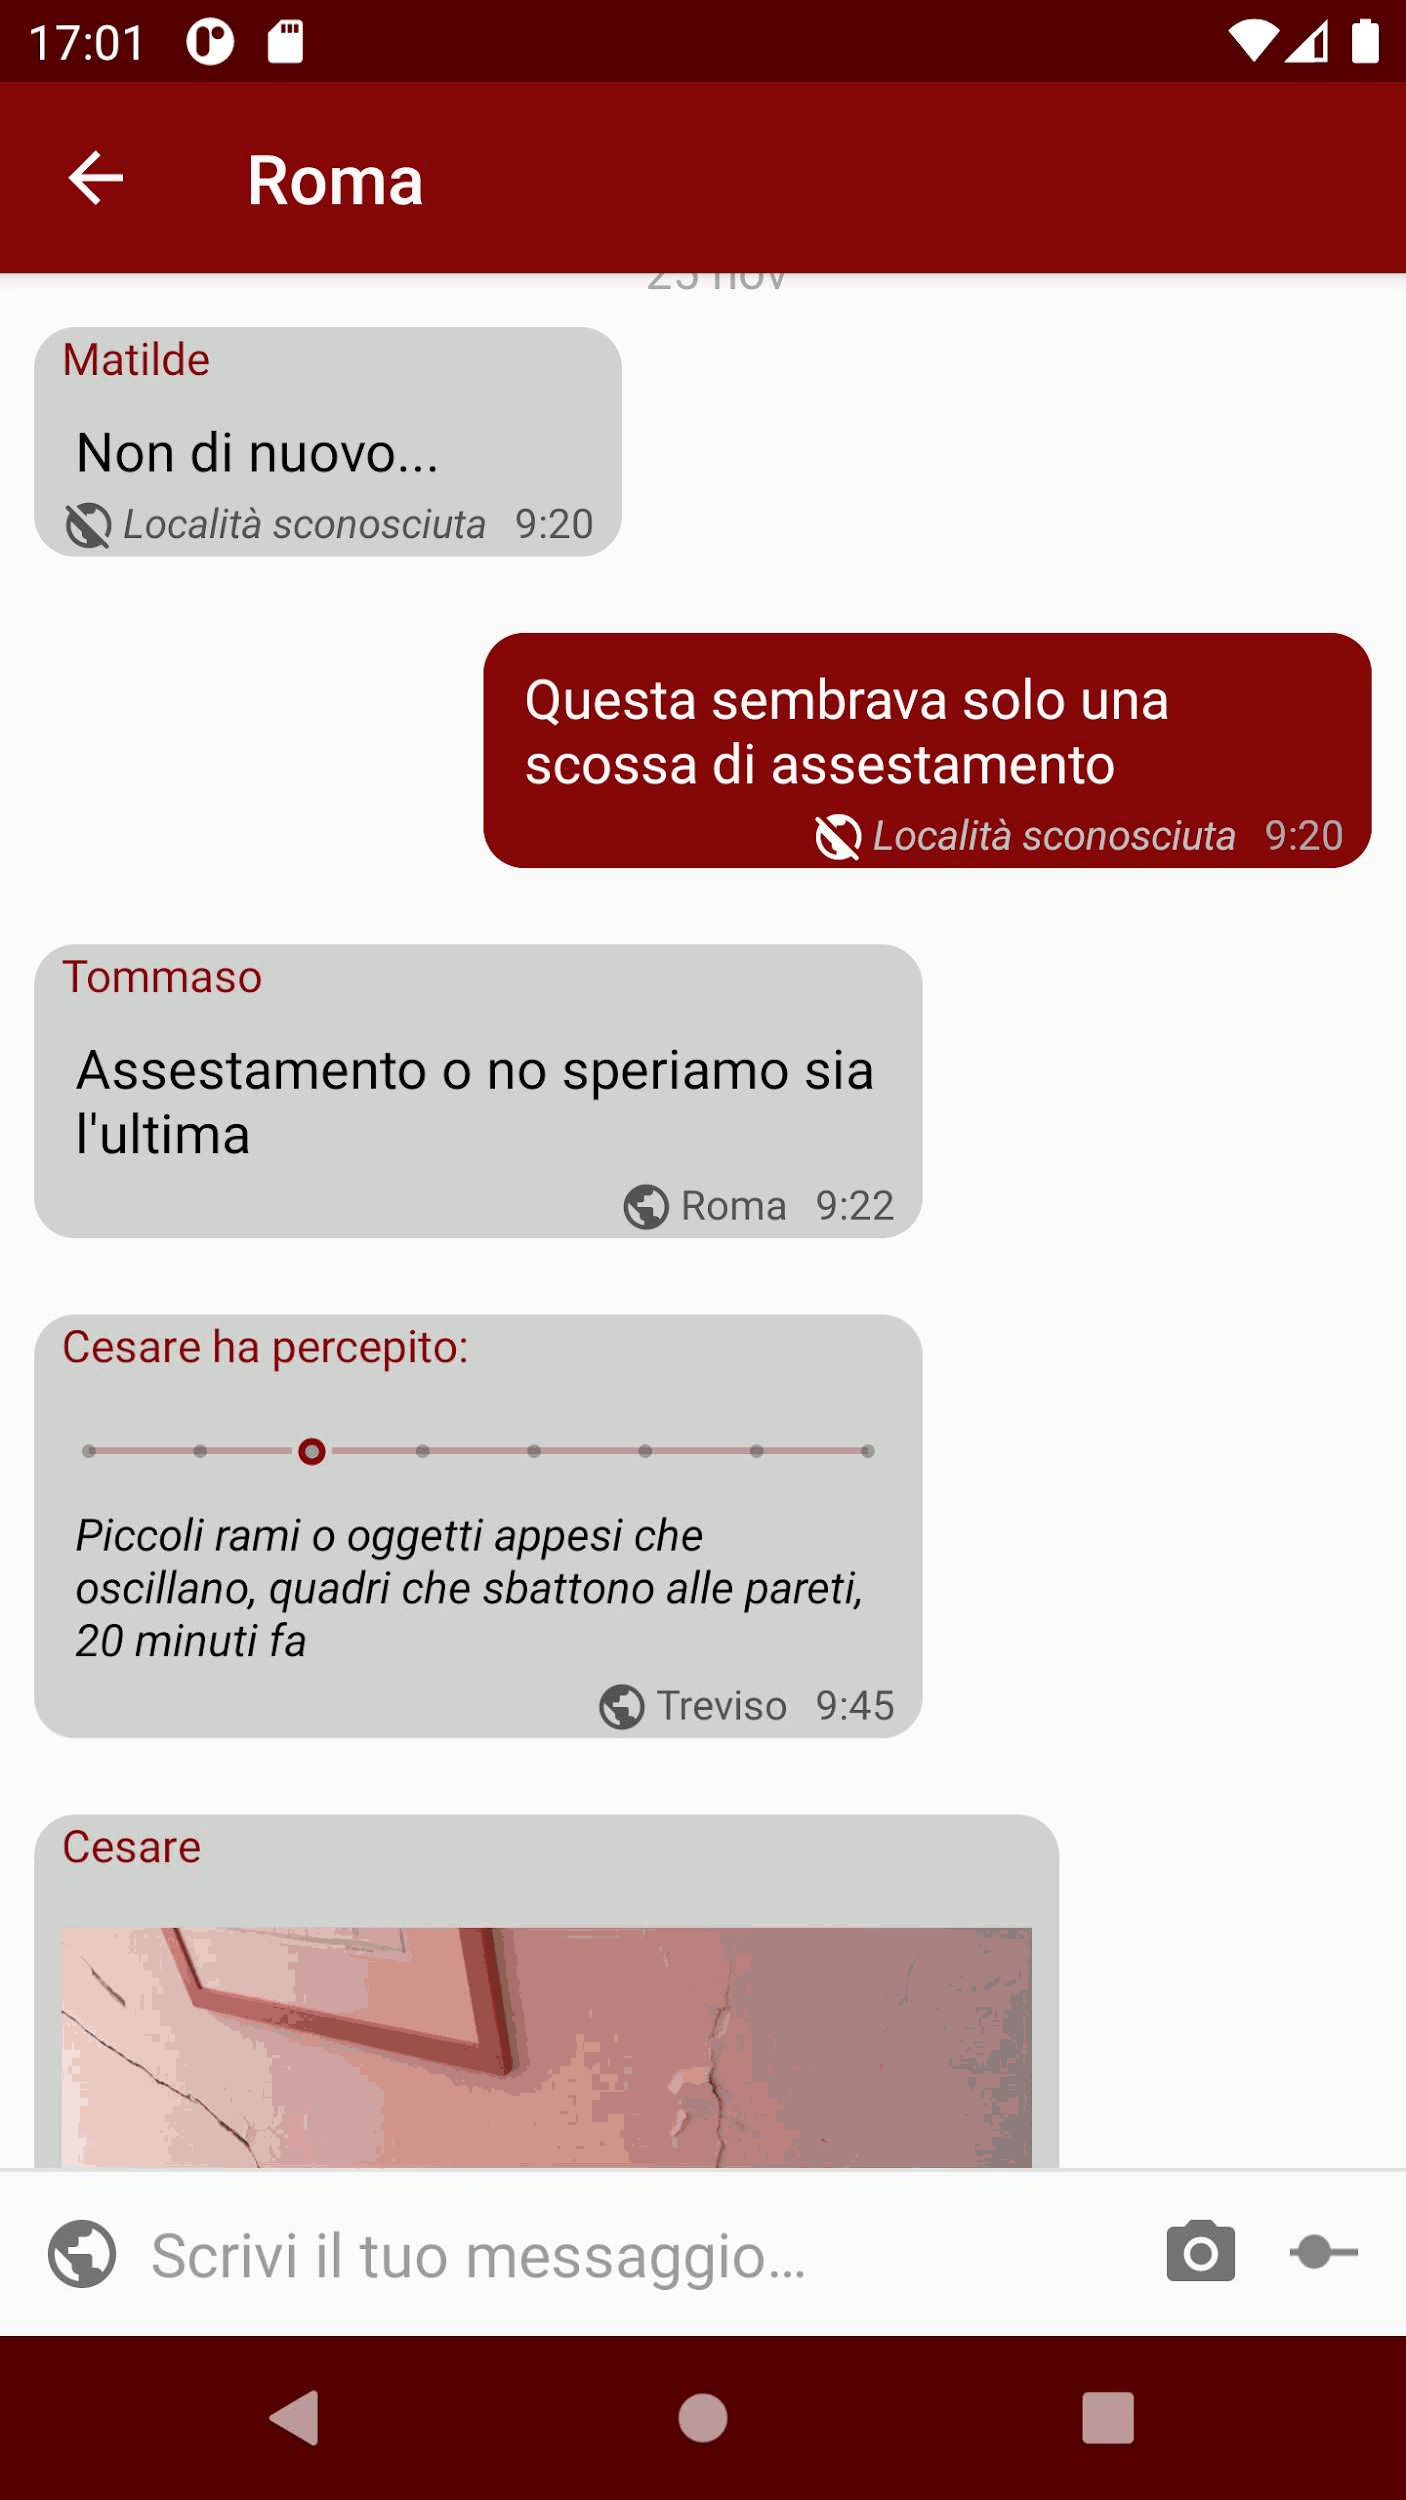
\includegraphics[width=0.85\linewidth]{assets/02/chat.png}
\caption{Schermata visualizzazione chat.}
\label{fig:android_chat}
\end{minipage}

\end{figure}

\begin{figure}[p]
\centering

\begin{minipage}{0.45\linewidth}
\centering
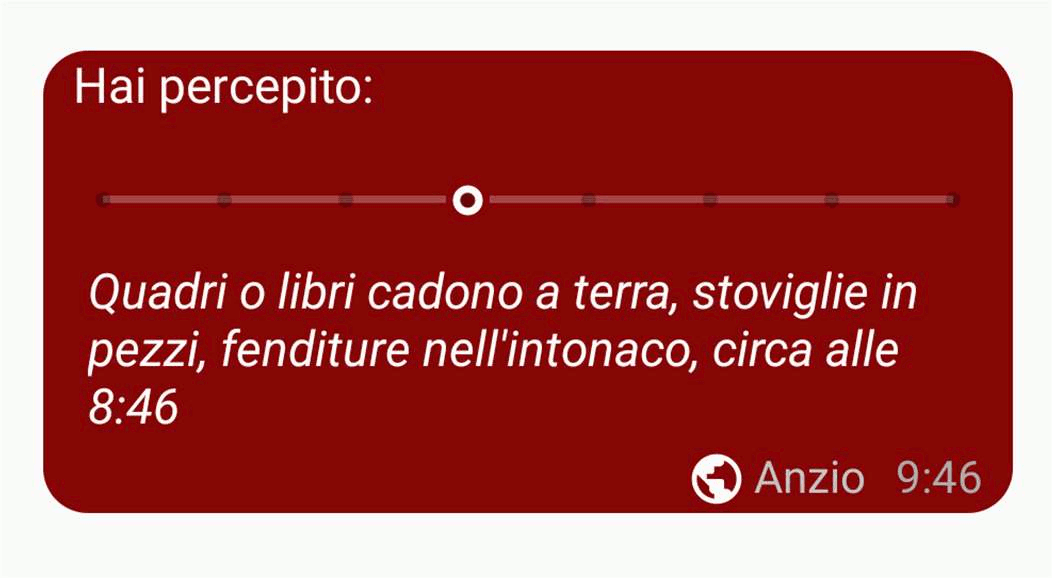
\includegraphics[width=0.85\linewidth]{assets/02/slider.png}
\caption{Dettaglio di un messaggio di tipo slider.}
\label{fig:android_slider}
\end{minipage}\hfill
\begin{minipage}{0.45\linewidth}
\centering
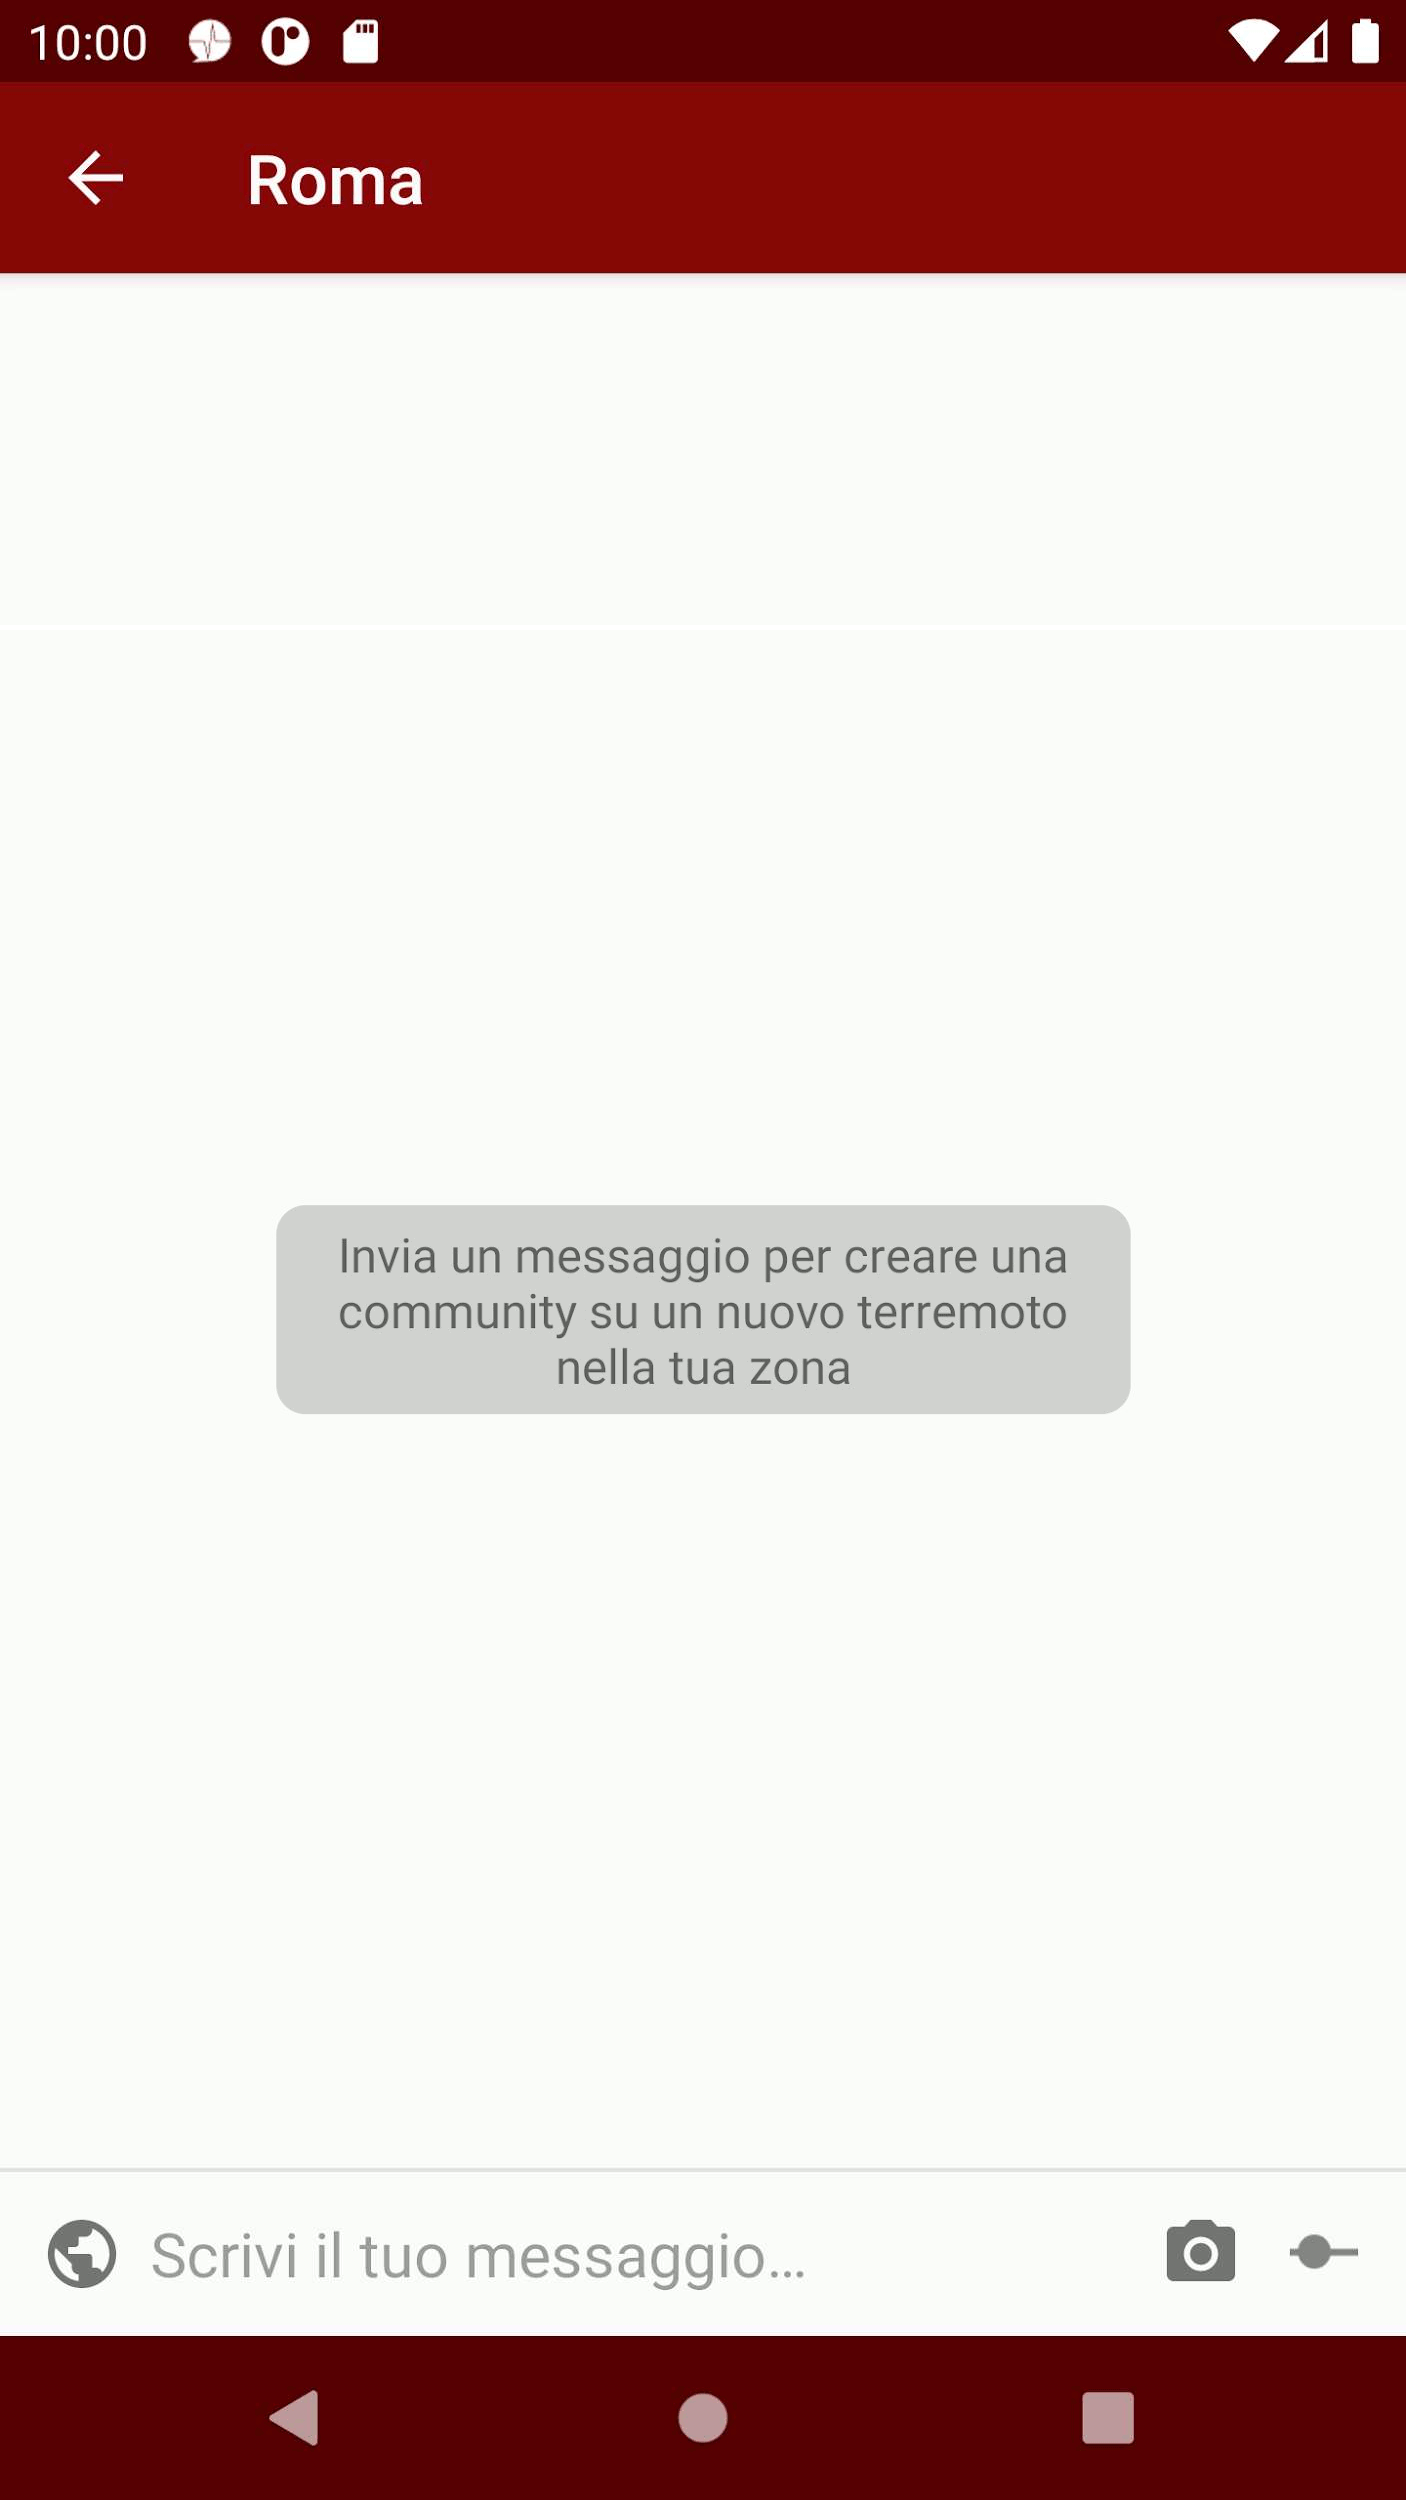
\includegraphics[width=0.85\linewidth]{assets/02/nuova_chat.png}
\caption{Schermata creazione di una chat.}
\label{fig:android_creazione}
\end{minipage}

\end{figure}

\section{Modellazione}

Il lavoro di Michele Spina lascia molte questioni aperte sulla funzionalità che vanno affrontate nella modellazione, progettazione e implementazione di una versione minimale ma effettivamente funzionante.

\paragraph{Dimensioni del modello} Una considerazione generale è stata fatta è sulle dimensioni del modello e quindi del numero di funzionalità da sviluppare. Si è preferito modellare e sviluppare un sistema piccolo ma completo, che soddisfi i principali requisiti, rispetto a uno complesso ma ricco di dettagli e funzioni. La ragione è quella di ottenere feedback da parte degli utenti in modo da estendere passo dopo passo il sistema.

\paragraph{Chat} Le chat sono degli spazi pubblici che contengono messaggi e che gli utenti possono accedere ed eventualmente interagire. La figura \ref{fig:chat_ciclo} mostra il ciclo di vita di una chat: nel momento della sua creazione non è \textit{verificata}, cioè non è stata associata con alcun terremoto; se, entro un termine di tempo specificato, viene effettuata questa associazione, passa nello stato di verificata, altrimenti viene chiusa. Quando una chat è chiusa diventa nascosta agli utenti e non è possibile inviare dei messaggi.

Un fatto importante è che nell'elenco delle chat vengono mostrate solo quelle aperte e solo quelle aggiornate di recente. Significa che l'utente non può scorrere la cronologia completa delle chat. Questa scelta insieme all'associazione con un terremoto derivano dall'obiettivo di tale funzionalità: permette l'interazione nel contesto delle scosse sismiche, scostandosi da un sistema di messaggistica generico.

\begin{figure}[ht!]
\centering
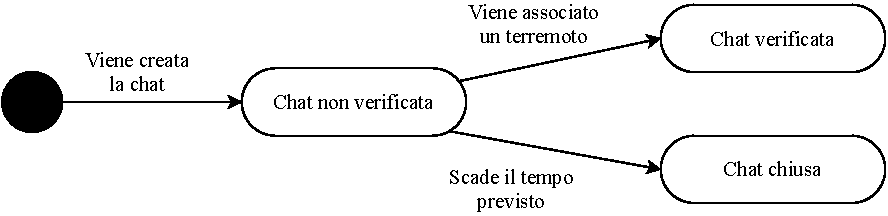
\includegraphics[width=\textwidth]{assets/02/chat_ciclo.pdf}
\caption{Ciclo di vita di una chat.}
\label{fig:chat_ciclo}
\end{figure}

\paragraph{Creazione di una chat} Viene definita una semplice regola per determinare quando una chat deve essere creata o meno: nel momento in cui l'utente richiede la creazione, il sistema analizza tutte le chat create in un arco specifico di tempo prima della richiesta (di solito qualche ora, visto che i terremoti non sono molto frequenti e che più scosse sismiche di un luogo possono essere accorpati in un unico terremoto), quindi per ognuna controlla che la distanza geografica rientri in un'area con centro le coordinate fornite nella richiesta (motivo per cui è obbligatorio che l'utente condivida la posizione) e un raggio specificato a livello di sistema. Se una chat esistente ha riscontro, viene rifiutata la richiesta e indirizzato l'utente sul quella che ha fatto riscontro. La regola pensata è primitiva, ma facilmente estendibile per migliorare la scelta di creazione.

\paragraph{Il ruolo della posizione geografica} Per una chat vengono salvate soltanto le coordinate geografica dell'utente che la crea. Da tali coordinate viene inferito il nome della chat, ponendo attenzione sui capoluoghi di provincia e sulla regione. L'associazione con un terremoto avviene confrontando i dati ufficiali provenienti da INGV \cite{ingv-data} con quelli della chat. Tale associazione non è precisa, è stato comunque deciso per il momento di non complicare ulteriormente il modello, per esempio considerando più coordinate geografiche.

La generazione del nome della chat viene effettuato tramite Nominatim \cite{nominatim}, il sistema fornito da OpenStreetMap per effettuare la geolocalizzazione partendo dalle coordinate geografiche o da un nome (come un indirizzo, una città o una regione).

\paragraph{Messaggi} L'utente può inviare un messaggio in una chat che non è stata chiusa. I tipi di messaggi sono quelli descritti nella sezione precedente. All'interno di una chat un utente può scorrere la cronologia completa dei messaggi. Il sistema rifiuterà messaggi testuali o fotografici che superano i limiti di dimensioni imposto a livello globale.

\paragraph{Username} L'utente per poter inviare un messaggio deve impostare un nome utente non univoco nel sistema. Gli utenti possono riconoscere altri utenti tramite questi nomi, ma non è possibile identificarli in modo univoco poiché i nomi utenti possono essere cambiati.

\paragraph{Sottoscrizioni} L'utente può iscriversi a una chat per ricevere le notifiche dei messaggi inviati. L'iscrizione è automatica nel momento in cui l'utente crea una chat. C'è possibilità di rimuovere un'iscrizione.

\paragraph{Il client} Il modello appena descritto, pur se minimale, si concentra principalmente sui comportamenti e caratteristiche lato server. Dall'altra parte, nel lato client, si aprono molte possibilità non esplorate in questo modello. In alcuni casi l'intervento del server aiuta nell'implementazione di funzionalità aggiuntive lato client, un esempio è l'anteprima dei messaggi che è prevista, mentre il contatore dei messaggi non letti non è previsto per il momento.


\chapter{Progettazione}
\label{ch:progg}

Il lavoro di progettazione è diviso in due parti strettamente collegate: prima la definizione delle API, che vengono esposta al client, dopo la progettazione del database. Durante le fasi di implementazione e test è spesso capitato di raffinare dettagli riguardo sia le API che il database, tuttavia il grosso del lavoro è stato svolto prima dell'implementazione.

\section{API}

Gli utenti possono interagire con SeismoCloud utilizzando l'applicazione mobile o l'applicazione Web. Tali applicazioni comunicano con il server utilizzando il protocollo HTTPS, seguendo lo stile architetturale REST. Affinché sia comprensibile le ragioni dietro la progettazione delle API, viene descritta brevemente l'architettura REST e lo strumento di progettazione vero e proprio, cioè la specifica OpenAPI.

\paragraph{Architettura REST} La \textit{representational state transfer} (REST) \cite{rest} è uno stile architetturale basato su HTTP \cite{http}. Un sistema di definisce \textit{RESTful} se implementa lo stile architetturale REST. Pur non essendo uno standard, un sistema \textit{RESTful} utilizza degli standard, nel caso di SeismoCloud: HTTP per la comunicazione, URI \cite{uri} per l'identificazione della risorsa e JSON \cite{json} per la rappresentazione della risorsa.

Affinché un sistema sia definibile \textit{RESTful}, è necessario che rispetti sei vincoli, di cui uno opzionale. Di seguito viene dato l'elenco e viene indicato come e se SeismoCloud soddisfa i vincoli, considerando sia le API già esistenti sia quelle progettate per l'occasione:

\begin{itemize}
\item \textbf{Client-server}: il client e il server devono essere dei sistemi indipendenti, uniti tramite delle interfacce. Poiché SeismoCloud effettua questa divisione tra client e server, soddisfa il vincolo.
\item \textbf{Stateless}: la comunicazione tra client e server non prevede il concetto di sessione. HTTPS è un protocollo di sua natura senza concetto di sessione, per cui tutte le informazioni necessarie al client o al server per soddisfare una richiesta sono contenute all'interno della singola comunicazione. SeismoCloud, e quindi le API, soddisfa questo vincolo.
\item \textbf{Cacheable}: le risposte del server devono essere costruite in modo da facilitare il loro riutilizzo, attraverso l'uso della cache (a livello del client o del server). SeismoCloud soddisfa questo vincolo, anche se alcune risposte delle API, in particolare quelle che dipendono dal tempo o dal singolo utente, non sono pensate per essere riutilizzate.
\item \textbf{Layered system}: il client non può sapere se è connesso direttamente al server che eroga le API o a un sistema intermedio. Nell'architettura di SeismoCloud, pur se non mostrato nella figura \ref{fig:architettura}, sono presenti dei server intermedi prima che una richiesta raggiungano gli applicativi che erogano effettivamente le API, per cui soddisfa il vincolo.
\item \textbf{Uniform interface}: letteralmente indica che le interfacce devono essere uniformi. Può significare molte cose, tra cui l'indipendenza tra il come vengono salvati i dati in un database e come vengono erogati al client, oppure la condizione per cui ogni API sia processabile in modo indipendente. SeismoCloud, come si vedrà anche in seguito, soddisfa questo vincolo.
\item \textbf{Code on demand}: l'unico vincolo \textbf{opzionale}, prevede di estendere o personalizzare le funzionalità di un client trasferendo codice eseguibile. SeismoCloud non soddisfa questo vincolo.
\end{itemize}

REST si basa sull'esistenza di risorse, che possono essere documenti o file identificati da un URL. Il client può accedere alla risorsa fornendo l'URL che la identifica e un'operazione da applicare, che corrispondono ai metodi HTTP (i più comuni sono \texttt{GET}, \texttt{POST}, \texttt{PUT}, \texttt{DELETE}). Nella realtà il client accede a una rappresentazione della risorsa, che può avvenire in varie forme in base al \textit{media type}, una stringa che identifica il formato che rappresenta la risorsa (a esempio JSON o XML). Solitamente le risorse sono organizzate in collezioni e il client può agire su quest'ultimo oltre che sulle risorse.

La tabella \ref{tab:rest} mostra la relazione tra i metodi HTTP e URL \cite{http-methods}. SeismoCloud segue questa relazione, l'unica differenza importante è che le API utilizzano il metodo \texttt{PUT} al posto di \texttt{POST} quando si agisce sulle collezioni. Questa caratteristica del sistema è stata seguita anche nelle API progettate, pur mantenere una consistenza interna anche se concettualmente errata.

\texttt{https://api.example.com/chats/} è un esempio di URL che identifica una collezione, \texttt{https://api.example.com/chats/3423} identifica una specifica risorsa all'interno della collezione.

\begin{table}[h!]
\centering
\caption{Semantica dei metodi HTTP e URL.}
\label{tab:rest}

\begin{tabular}{c|p{14em}|p{14em}}
\textbf{Metodo} & \textbf{URL collezione} & \textbf{URL risorsa} \\
\hline
GET & Restituisce l'elenco delle risorse. & Restituisce la risorsa. \\
PUT & Sostituisce l'intera collezione. & Sostituisce o crea la risorsa. \\
POST & Crea una risorsa nella collezione. & Vedi PUT. \\
DELETE & Elimina l'intera collezione. & Elimina la risorsa. \\
\end{tabular}
\end{table}

\paragraph{OpenAPI} Il frammento di codice \ref{listing:openapi} mostra come viene definita nella specifica OpenAPI 3.0 \cite{openapi}, conosciuta in origine come specifica Swagger, l'API \texttt{GET /seismometers/}. Tale specifica permette di progettare API RESTful in modo \textit{machine-readable format}, cioè che siano processabili dal computer. I software che implementano la specificano possono essere utilizzati per diversi scopi, tra cui la generazione automatica di codice implementativo o di test, il controllo semantico delle API, la generazione della documentazione in vari formati e molto altro. In SeismoCloud OpenAPI viene utilizzato per fini documentativi. Il vantaggio principale è che le API possono essere progettate e documentate in un semplice file testuale, modificabile da qualsiasi editor di testo e convertibile in altri formati. La figura \ref{fig:openapi-render} mostra la conversione automatica dalla specifica a codice HTML per la documentazione.

In SeismoCloud il file della specifica è realizzato in formato standard YAML \cite{yaml} e utilizza versione 3.0 della specifica. Per ogni URL vengono elencate le operazioni (\texttt{GET}, \texttt{POST}...) e per ognuna si specificano gli eventuali parametri nel percorso o nella query, l'eventuale body e le possibili risposte. Quando si coinvolgono degli schemi, come mostrato nel frammento in \texttt{callback}, OpenAPI utilizza un sottoinsieme arricchito della specifica JSON Schema \cite{json-schema}, per indicare il tipo, la lunghezza o altre caratteristiche del dato.

\afterpage{\clearpage} % Aiuta il posizionamento dei float.

\begin{figure}[ht]
\centering
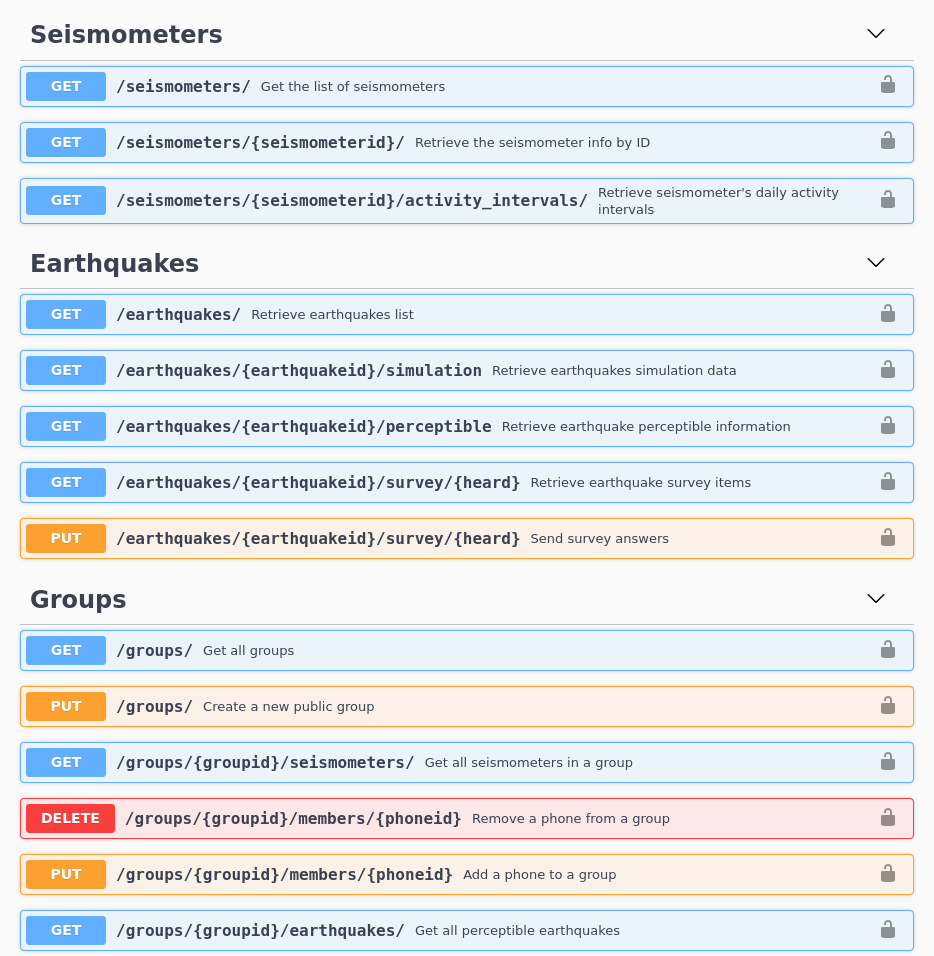
\includegraphics[width=\textwidth]{assets/03/openapi.png}
\caption{Conversione del file testuale delle API in HTML.}
\label{fig:openapi-render}
\end{figure}

\begin{longlisting}
\begin{minted}{yaml}
paths:
  # Seismometers
  /seismometers/:
    parameters:
      - $ref: "#/components/parameters/XPhoneID"
      - $ref: "#/components/parameters/XAppBuild"
      - $ref: "#/components/parameters/XAppVersion"
      - $ref: "#/components/parameters/XAppLanguage"
      - $ref: "#/components/parameters/XAppPlatform"
    get:
      tags: ["Seismometers"]
      operationId: getSeismometers
      summary: Get the list of seismometers
      description: |-
        The response contains the list of all seismometers. If the user is not
        the owner of the sensor, the position might be scrambled due to privacy
        flag.
      security:
        - OpenID: []
      parameters:
        - name: callback
          in: query
          schema: { type: string }
          required: false
          description: Callback JSONP function name
      responses:
        '200':
          description: Seismometer list available
          content:
            application/json:
              schema:
                type: array
                items:
                  $ref: '#/components/schemas/Seismometer'
        '400': { $ref: '#/components/responses/BadRequest' }
        '500': { $ref: '#/components/responses/InternalServerError' }
\end{minted}
\caption{Specifica di \texttt{GET /seismometers/} in OpenAPI 3.0.}
\label{listing:openapi}
\end{longlisting}

\paragraph{API} Per implementare la funzionalità di messaggistica sono state progettate 9 API REST, riassunte nella tabella \ref{tab:api}. Le risorse esposte al client sono le chat, il nome utente, i messaggi e le sottoscrizioni. Su tali risorse e relative collezioni il client non può operare con tutti i metodi, ma solo con quelli permessi.

Sono state seguite strettamente le convenzioni utilizzate nelle altre API di SeismoCloud, ciò ha influito la scelta dei codici di stato restituiti, la formazione dei percorsi, l'uso del metodo \texttt{PUT} al posto di \texttt{POST} nella creazione di risorse all'interno di una collezione (per esempio in \texttt{PUT /chats/\{chatid\}/messages/}).

\begin{table}[ht!]
\centering
\caption{Elenco riassuntivo delle API progettate.}
\label{tab:api}

\begin{tabular}{c|c|p{16em}}
\textbf{Metodo} & \textbf{URL} & \textbf{Descrizione} \\
\hline
GET & /chats/ & Restituisce un elenco delle ultime chat aggiornate. \\
PUT & /chats/ & Crea una nuova chat. \\
GET & /chats/\{chatid\}/messages/ & Restituisce un elenco dei messaggi della chat. \\
PUT & /chats/\{chatid\}/messages/ & Crea un messaggio in una chat. \\
GET & /images/\{imageid\} & Recupera l'immagine. \\
GET & /me/username & Recupera il nome utente. \\
PUT & /me/username & Imposta il nome utente. \\
DELETE & /me/chats/subscribed/\{chatid\} & Elimina la sottoscrizione a una chat. \\
PUT & /me/chats/subscribed/\{chatid\} & Crea la sottoscrizione a una chat.
\end{tabular}
\end{table}

\paragraph{Schemi} In aggiunta alle API sono stati definiti gli schemi che possono essere restituiti o che il client deve inserire nella chiamata affinché vada a buon fine. Gli schemi consistono in tipi primitivi, come interi e stringe, o composti, come oggetti e liste. Affinché il client utilizzi in modo corretto le API è importante definire e documentare tali schemi. La tabella \ref{tab:schemi} riassume tutti gli schemi utilizzati nelle API sopracitate.

I tipi primitivi \texttt{EarthquakeID}, \texttt{Latitude} e \texttt{Longitude} sono già preesistenti nel progetto, mentre gli altri sono stati definiti per l'occasione. I tipi primitivi, come \texttt{SliderValue} o \texttt{TextValue}, sono specializzazioni dei tipi come interi o stringhe.

Gli unici tipi composti disponibili sono gli oggetti \texttt{Message} e \texttt{Chat}, con gli attributi mostrati nella tabella \ref{tab:chat_message}. In \texttt{Message}, Il client può distinguere il tipo del messaggio controllando l'attributo \texttt{type} per poi accedere all'attributo corrispondente al tipo. In caso di un'immagine viene indicato il suo identificativo per ottenere l'immagine con \texttt{GET /images/\{imageid\}}. In \texttt{Chat}, l'attributo \texttt{latestMessage} è opzionale perché una chat appena creata potrebbe non contenere alcun messaggio; la funzione di tale attributo è permettere l'anteprima del messaggio nell'elenco delle chat. L'attributo \texttt{eartquakeID} è opzionale perché una chat potrebbe non avere associato alcun terremoto. Non è possibile inviare un messaggio in una chat chiusa. Le coordinate indicano la zona approssimativa in cui la chat è stata creata.

\begin{table}[ht!]
\centering
\caption{Elenco riassuntivo schemi utilizzati dalle API.}
\label{tab:schemi}

\begin{tabular}{c|c|c|p{14em}}
\textbf{Nome} & \textbf{Tipo} & \textbf{Formato} & \textbf{Descrizione} \\
\hline
ChatID & \texttt{integer} & \texttt{int64} & Identificativo di una chat. \\
MessageID & \texttt{integer} & \texttt{int64} & Identificativo di un messaggio. \\
ImageID & \texttt{string} & \texttt{UUID} & Identificativo di un'immagine. \\
EarthquakeID & \texttt{integer} & \texttt{int64} & Identificativo interno di un terremoto. \\
Latitude & \texttt{number} & --- & Latitudine in gradi. \\
Longitude & \texttt{number} & --- & Longitudine in gradi. \\
Username & \texttt{string} & --- & Nome utente mostrato nei messaggi. \\
SliderValue & \texttt{integer} & --- & Valore dello slider. \\
TextValue & \texttt{string} & --- & Contenuto di un messaggio testuale. \\
Image & \texttt{string} & \texttt{binary} & L'immagine in formato binario. \\
Message & \texttt{object} & --- & Singolo messaggio in una chat. \\
Chat & \texttt{object} & --- & Singola chat.
\end{tabular}
\end{table}

\afterpage{\clearpage}

\begin{table}[ht!]
\centering
\caption{Attributi degli schemi \texttt{Chat} e \texttt{Message}.}
\label{tab:chat_message}

\begin{tabular}{c|c|c|p{17em}}
\hline
\multicolumn{4}{c}{\textbf{\texttt{Message}}} \\
\hline
\textbf{Nome} & \textbf{Tipo} & \textbf{Formato} & \textbf{Descrizione} \\
\hline
id & \texttt{MessageID} & --- & Obbligatorio, identificativo di un messaggio. \\
createdAt & \texttt{string} & \texttt{date-time} & Obbligatorio, data e ora di invio del messaggio. \\
sentBy & \texttt{Username} & --- & Obbligatorio, nome utente di chi ha inviato il messaggio. \\
type & \texttt{string} & \texttt{enum} & Obbligatorio, con valori possibili \texttt{text}, \texttt{image} o \texttt{slider}, indica il tipo del messaggio inviato. \\
text & \texttt{TextValue} & --- & Contenuto testuale, che può essere un messaggio di testo o l'identificativo di un'immagine. \\
slider & \texttt{SliderValue} & --- & Valore dello slider.
\end{tabular}

\bigskip

\begin{tabular}{c|c|c|p{17em}}
\hline
\multicolumn{4}{c}{\textbf{\texttt{Chat}}} \\
\hline
\textbf{Nome} & \textbf{Tipo} & \textbf{Formato} & \textbf{Descrizione} \\
\hline
id & \texttt{ChatID} & --- & Obbligatorio, identificativo di una chat. \\
name & \texttt{string} & --- & Obbligatorio, nome della chat. \\
createdAt & \texttt{string} & \texttt{date-time} & Obbligatorio, data e ora di creazione della chat. \\
closed & \texttt{boolean} & --- & Obbligatorio, indica se la chat è stata chiusa. \\
subscribed & \texttt{boolean} & --- & Obbligatorio, indica se l'utente è sottoscritto alla chat. \\
latitude & \texttt{Latitude} & --- & Obbligatorio. \\
longitude & \texttt{Longitude} & --- & Obbligatorio. \\
earthquakeID & \texttt{EarthquakeID} & --- & Indica il terremoto associato. \\
latestMessage & \texttt{Message} & --- & Ultimo messaggio inviato. \\
\end{tabular}
\end{table}

\paragraph{Rappresentazione delle risorse} \texttt{Content-Type} è il parametro header utilizzato per indicare la rappresentazione della risorsa o della collezione. Il valore di tale parametro si chiama \textit{media type} \cite{mediatype-ass,mediatype-spec}. Tutte le API che restituiscono una risorsa o una collezione utilizzano il media type \texttt{application/json}, tranne per \texttt{GET /images/\{imageid\}} che restituisce l'immagine in formato binario \texttt{image/jpeg}. Solo le API \texttt{PUT /me/username} e \texttt{PUT /chats/\{chatid\}/messages} prevedono l'uso del body nella richiesta. Nel primo caso \texttt{Content-Type} deve essere \texttt{text/plain}, mentre nel secondo caso il tipo di messaggio da inviare viene riconosciuto con tre diversi media type:

\begin{itemize}
\item \texttt{text/x.slider}: messaggio slider di tipo \texttt{SliderValue}. Questo media type è personalizzato e vale solo in SeismoCloud. 
\item \texttt{text/plain}: messaggio testuale di tipo \texttt{TextValue}.
\item \texttt{image/jpeg}: messaggio con immagine, di tipo \texttt{Image}.
\end{itemize}

\paragraph{Parametri obbligatori} Il client per poter utilizzare le API è necessario che inserisca cinque parametri nell'header della richiesta. Tali parametri sono elencati nella tabella \ref{tab:header_obbligatori}. L'uso di questi parametri dipende dalle necessità della API utilizzata, per esempio in base alla versione dell'applicazione il server può comportarsi in modi differenti, o restituire dei risultati in base alla lingua indicata. Pur essendo obbligatori per il client, il server è libero di utilizzarli, infatti nel caso del servizio di messaggistica sono ignorati.

\begin{table}[ht!]
\centering
\caption{Parametri header obbligatori per tutte le API.}
\label{tab:header_obbligatori}

\begin{tabular}{c|c|p{19em}}
\textbf{Nome} & \textbf{Tipo} & \textbf{Descrizione} \\
\hline
\texttt{X-PHONE-ID} & \texttt{string} & Identificativo del telefono. \\
\texttt{X-APP-BUILD} & \texttt{integer} & Numero di build dell'applicazione. \\
\texttt{X-APP-VERSION} & \texttt{string} & Numero di versione sematica dell'applicazione. \\
\texttt{X-APP-LANG} & \texttt{string} & Lingua utilizzata in formato ISO 639-1. \\
\texttt{X-APP-PLATFORM} & \texttt{string} & Sistema operativo (Android o iOS).
\end{tabular}
\end{table}

\paragraph{Autenticazione} Solo un numero ristretto di API possono essere utilizzate senza autenticazione. Nel caso del servizio di messaggistica è necessario che il client sia autenticato tramite Keycloak. Il client autenticato ottiene un token che passerà alle API con il parametro \texttt{Authorization} nell'header della richiesta. Il server si limiterà a validare il token e a estrarre da esso informazioni utili, tra cui l'\texttt{UserID}. Per il token Keycloak segue lo standard JSON Web Token \cite{json-token}.

\paragraph{Codici di stato} Tutte le API mostrate restituiscono codici di stato che seguono standard HTTP. I codici comunemente restituiti sono elencati nella tabella \ref{tab:codici_stato}. In aggiunta sono stati definiti dei codici personalizzati \texttt{399}, \texttt{498} e \texttt{499} per indicare degli errori contestualizzati all'interno di SeismoCloud. 

La differenza tra i codici di stato \texttt{200} e \texttt{201} nel caso di SeismoCloud non è netta, poiché il metodo \texttt{PUT} viene utilizzato anche quando normalmente andrebbe \texttt{POST}. Si è deciso di caso in caso quando restituire \texttt{200} o \texttt{201}.

\begin{table}[ht!]
\centering
\caption{Codici di stato comunemente restituiti dalle API.}
\label{tab:codici_stato}

\begin{tabular}{c|c|p{19em}}
\textbf{Codice} & \textbf{Frase esplicativa} & \textbf{Descrizione} \\
\hline
200 & OK & La richesta è andata a buon fine. \\
201 & Created & La risorsa è stata creata. \\
399 & Chat already created & La chat è stata già creata. \\
400 & Bad Request & La richiesta è malformata. \\
401 & Unauthorized & Il client non è autorizzato. \\
404 & Not Found & La risorsa indicata non è stata trovata. \\
498 & Chat closed & La chat è stata chiusa. \\
499 & Username required & L'utente non ha impostato il nome utente. \\
500 & Internal Server Error & Il server ha riscontrato un errore. \\
\end{tabular}
\end{table}

\paragraph{Comportamento di \texttt{PUT /chats/}} Tra tutte le API, \texttt{PUT /chats/} è speciale poiché la logica di creazione della chat dipende dai fattori descritti nel capitolo precedente. Se il server decide che la chat non va creata, perché ne esiste una potenzialmente simile, la chiamata restituisce il codice di stato \texttt{399} insieme alla chat già esistente, altrimenti crea la chat e la restituisce con codice di stato \texttt{201}.

\section{Database}

Per progettare il database sono stati seguiti tre passaggi. Il primo consiste nella realizzazione di un diagramma concettuale entità-associazione che descrive il dominio di interesse in modo chiaro e senza restrizioni o modelli imposti dal database. Il secondo passo consiste nella ristrutturazione del diagramma in uno più vicino al modello relazionale. Infine il terzo passaggio consiste nella conversione immediata del diagramma nel codice implementativo SQL, specifico per il database MariaDB, database che è attualmente utilizzato in SeismoCloud.

\begin{wrapfigure}{r}{0.5\textwidth}
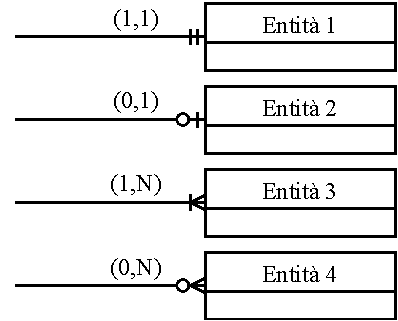
\includegraphics{assets/03/crow.pdf}
\caption{Notazione \textit{Crow's foot}.}
\label{fig:crow}
\end{wrapfigure}

\paragraph{Notazione Crow's foot} Per la realizzazione del diagramma concettuale e relazionale è stata utilizzata la notazione \textit{Crow's foot}, che rappresenta le entità come rettangoli, le quali possono avere degli attributi, e le associazioni come linee che collegano i rettangoli. La cardinalità e l'opzionalità delle associazioni si può indicare con una combinazione di specifici simboli alle estremità delle linee. I simboli utilizzati sono: l'\textbf{anello} che indica l'opzionalità, la \textbf{linea} che indica la molteplicità singola e la \textbf{zampa} che indica la molteplicità multipla. Tali simboli possono essere combinati per formare quattro tipologie di cardinalità mostrate nella figura \ref{fig:crow}. Nei diagrammi progettati vengono utilizzate tutte le cardinalità tranne la (1, N).

\paragraph{Differenza dei diagrammi} I due diagrammi, pur se sono esteticamente simili, svolgono funzioni diverse: il primo è un diagramma astratto del dominio di studio, che può essere implementato in modo diverso, per esempio in un database a oggetti o anche NoSQL, quindi non relazionale, mentre il secondo è un diagramma più vicino al database di riferimento, nel caso specifico relazionale. Il vantaggio di questa separazione è nella maggiore flessibilità nel primo diagramma, potendo esplorare e descrivere il dominio in maniera molto più libera.

\paragraph{Diagramma concettuale} La figura \ref{fig:diagramma_concettuale} mostra il diagramma concettuale, una visione ad alto livello che coinvolge soltanto entità, relazioni e attributi. In questo livello non è necessario specificare eventuali chiavi primarie, poiché verranno scelte nel passo successivo. Degli attributi elencati non viene specificata la cardinalità. Viene utilizzato il concetto di generalizzazione completa per l'entità \texttt{Message}: un'istanza di \texttt{Message} deve essere un'istanza esattamente di \texttt{Slider}, \texttt{Text} o \texttt{Image} in modo esclusivo. Rispetto alle altre entità, \texttt{Earthquake} è l'unica che è preesistente nel modello; i suoi attributi sono stati nascosti poiché non utilizzati.

\begin{figure}[ht!]
\centering
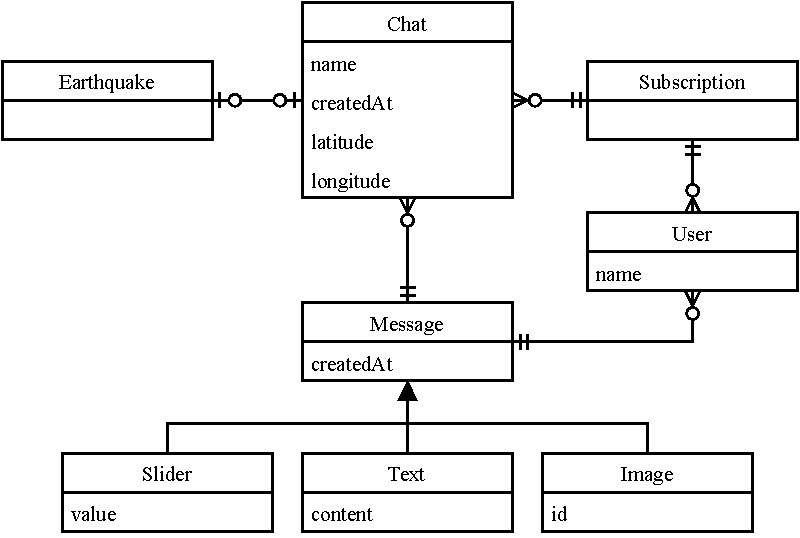
\includegraphics[width=\textwidth]{assets/03/concettuale.pdf}
\caption{Diagramma concettuale.}
\label{fig:diagramma_concettuale}
\end{figure}

\paragraph{Diagramma relazionale} Il diagramma concettuale è stato in seguito ristrutturato tenendo in mente il modello relazionale, in particolare quello implementato da MariaDB. In questo livello vengono specificate le cardinalità degli attributi, che sono del tipo (1,1) o (0,1) in base alla presenza o meno del simbolo \texttt{+}. Vengono assegnati i tipi degli attributi, senza però scendere a un livello troppo dettagliato. Sono state specificate le chiavi primarie per ogni relazione, indicando in caso di interi l'opzione di incremento automatico a ogni inserimento. Il risultato è mostrato nella figura \ref{fig:diagramma_relazionale}. Non essendo supportato il concetto di generalizzazione, si è deciso di unificare tutte le entità figlie di \texttt{Message} in una unica con l'attributo \texttt{type} che funziona da discriminante. Gli attributi \texttt{id} e \texttt{content} sono stati unificati, poiché assumono lo stesso tipo, cioè una stringa. Viene garantito, tramite l'aggiunta di un vincolo, che in base all'attributo discriminante, il corrispettivo \texttt{textcontent} o \texttt{intcontent} non sia nullo.

\paragraph{Codice SQL} Una volta ristrutturato il diagramma in modo da essere implementato in un database relazionale, la conversione in SQL è immediata. Il frammento di codice \ref{listing:diagramma_sql} mostra la conversione in SQL solo dell'entità \texttt{Chat}. Nella conversione, oltre a precisare la tipologia di dato in base alla disponibilità del database, sono state seguire le convenzioni utilizzate dalle altre tabelle in SeismoCloud, a esempio nei campi testuali e nella scelta del tipo per numeri a virgola mobile. Ogni colonna è stata rigorosamente commentata (non mostrato nel frammento), in modo da risultare il più possibile chiaro da parte di altre persone del team. Sono stati implementati direttamente in SQL i vincoli più semplici che coinvolgono la riga stessa; gli ulteriori vincoli complessi sono gestiti direttamente dall'applicativo.

\begin{listing}
\begin{minted}{sql}
CREATE TABLE `chat` (
    `id`           bigint unsigned AUTO_INCREMENT,
    `name`         varchar(255)                   NOT NULL,
    `createdat`    datetime                       NOT NULL,
    `closed`       boolean                        NOT NULL,
    `latitude`     double                         NOT NULL,
    `longitude`    double                         NOT NULL,
    `earthquakeid` int(10) unsigned,
    PRIMARY KEY (`id`),
    UNIQUE KEY (`earthquakeid`),
    CONSTRAINT `chatEarthquakeid` FOREIGN KEY (`earthquakeid`) REFERENCES `events` (`id`) ON DELETE CASCADE ON UPDATE CASCADE
) ENGINE=InnoDB DEFAULT CHARSET=utf8;
\end{minted}
\caption{Implementazione SQL del modello.}
\label{listing:diagramma_sql}
\end{listing}

\begin{figure}[ht!]
\centering
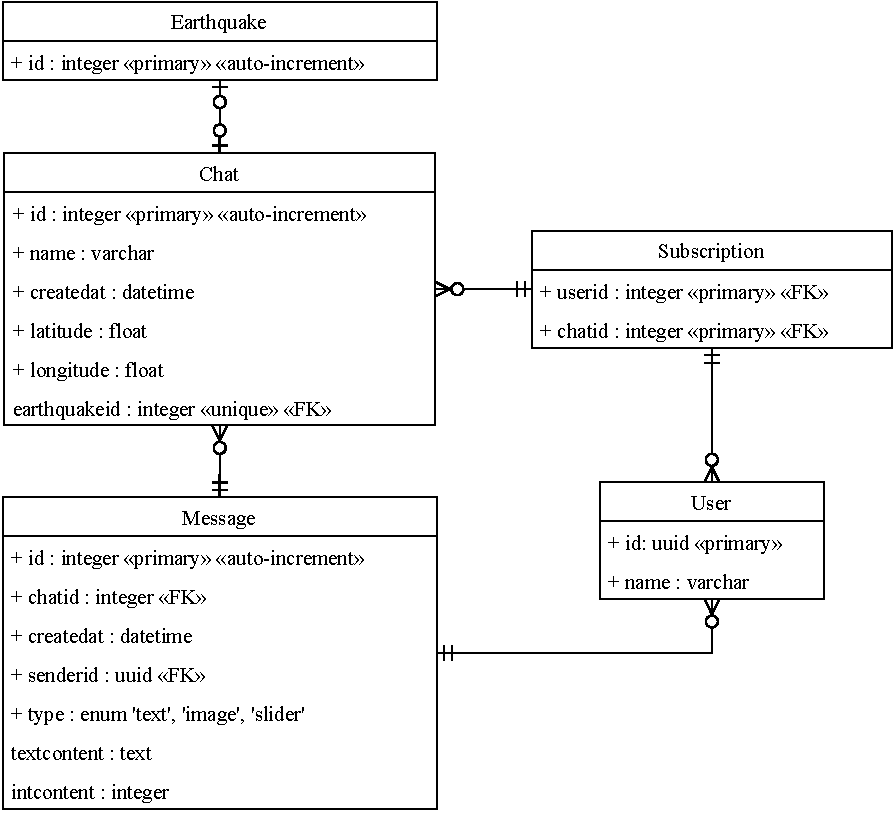
\includegraphics[width=\textwidth]{assets/03/relazionale.pdf}
\caption{Diagramma relazionale.}
\label{fig:diagramma_relazionale}
\end{figure}


\chapter{Implementazione}
\label{ch:impl}

La figura \ref{fig:architettura-modify} mostra i nodi in linea tratteggiata che sono stati modificati per implementare la funzionalità nell'architettura di SeismoCloud:

\begin{itemize}
\item \textbf{API principali}: sono state implementate le API progettate nel capitolo precedente;
\item \textbf{MariaDB}: sono state create le tabelle necessarie in SQL basandosi sulla progettazione del capitolo precedente;
\item \textbf{Worker}: sono stati aggiunti dei compiti periodici che sono separati dalle API, e quindi dall'interazione diretta con i client;
\item \textbf{MinIO}: è stato aggiunto un \textit{bucket} per conservare le immagini associate ai messaggi. Un bucket è un modo di organizzare gli oggetti simili alle cartelle di un filesystem, ma è un termine specifico per un object storage server com'è MinIO.
\item \textbf{Nominatim}: sono state implementate delle interfacce per interagire con il servizio esterno Nominatim tramite le API pubbliche. Il servizio è utilizzato per l'assegnazione di un nome di una chat nelle API principali e per l'associazione di una chat con il terremoto in Worker.
\end{itemize}

\begin{figure}[ht!]
\centering
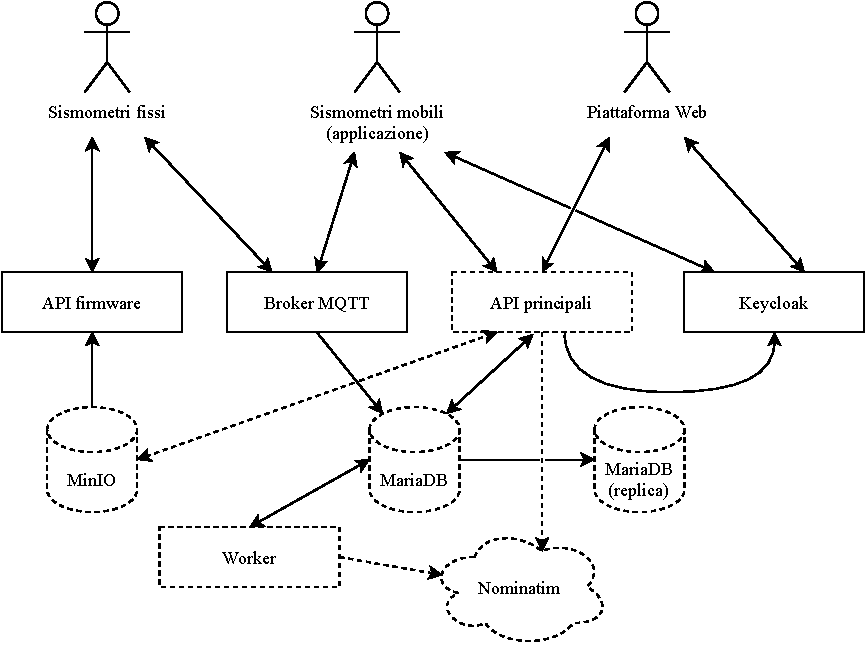
\includegraphics[width=\textwidth]{assets/04/architettura-modify.pdf}
\caption{Nodi coinvolti nell'implementazione della funzionalità.}
\label{fig:architettura-modify}
\end{figure}

Dal momento che MariaDB e MinIO sono software preesistenti, non hanno richiesto lavori di sviluppo poiché sono stati semplicemente configurati per la funzionalità. Lo sviluppo vero e proprio è invece avvenuto nelle API principali e nel Worker, due software realizzati in linguaggio Go. Per poter descrivere le sfide implementative e le scelte adottate durante il processo, è necessaria quindi una breve panoramica sul linguaggio e sull'organizzazione del codice backend di SeismoCloud.

\section{Il linguaggio Go}

\paragraph{Linguaggio Go} Go \cite{go}, il cui logo è mostrato nella figura \ref{fig:logo_go}, è un linguaggio di programmazione tipizzato staticamente e multi-paradigma, sintatticamente simile al C, che mira a una compilazione efficiente, un'esecuzione veloce e di una facile programmazione. Le due principali implementazioni sono un compilatore self-host, che prevede anche un insieme di strumenti per gestire un progetto in Go, e \texttt{gccgo}, la versione implementata per il compilatore GCC.

\begin{wrapfigure}{r}{0.30\textwidth}
\centering

\includegraphics[scale=0.20]{assets/04/logogo.png}
\caption{Logo di Go.}
\label{fig:logo_go}
\end{wrapfigure}

In Go è possibile programmare in paradigma orientato alla concorrenza, funzionale e imperativo, con una connotazione particolare per gli oggetti. Prevede dei meccanismi di sicurezza per la memoria, tra cui una gestione della memoria (\textit{garbage collection}, GC) e uno stile di concorrenza basato sullo scambio di messaggi attraverso dei canali. Il listato di codice \ref{listing:hello_world} mostra il classico programma dimostrativo in Go, che stampa un messaggio nell'output testuale. I principali utilizzi di Go sono per la costruzione di programmi che interagiscono con la rete o per programmi a riga di comando.

\paragraph{Go e SeismoCloud} In SeismoCloud Go è utilizzato per implementare le API esposte ai client e per i compiti periodici eseguiti in modo indipendente dalle API. Viene utilizzata l'ultima versione disponibile del linguaggio e della principale implementazione, la 1.16, che consiste in un compilatore e diversi strumenti aggiuntivi per la gestione del progetto.

\begin{listing}
\begin{minted}{go}
package main

import "fmt"

func main() {
	fmt.Println("Hello, World!")
}
\end{minted}
\caption{Classico programma dimostrativo ``Hello World!'' in Go.}
\label{listing:hello_world}
\end{listing}

\paragraph{Organizzazione del codice} Due concetti importanti in Go sono i \textit{moduli} e i \textit{package}. Un modulo è una collezione di package che sono sviluppati e distribuiti insieme, mentre un package è collezione di codici sorgenti in Go che risiedono nella stessa cartella. Un package può contenere a sua volta altri package. Il backend di SeismoCloud, d'ora in poi indicato solo con ``SeismoCloud'', è organizzato in una singola repository composta da un modulo e diversi package che suddividono il sistema in modo sia orizzontale che verticale. La figura \ref{fig:repository} mostra tale suddivisione. I package all'interno di \texttt{service} sono pensati per essere utilizzati in base alle necessità del singolo servizio. Un esempio è \textit{scsfilestorage}, responsabile dell'interazione con MinIO, utilizzato sia dalle API firmware che dalle API principali, nel primo caso per distribuire gli aggiornamenti ai firmware, nel secondo per distribuire le immagini. Invece quelli in \texttt{cmd} sono una suddivisione verticale, per cui \texttt{webapi} contiene il codice necessario per le API principali, mentre \texttt{worker} contiene il codice necessario per il Worker.

\begin{figure}[ht!]
\centering
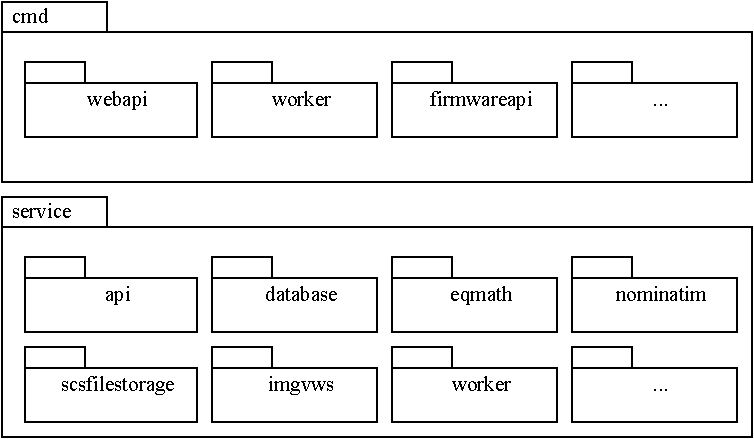
\includegraphics[width=0.8\textwidth]{assets/04/repository.pdf}
\caption{Organizzazione dei principali package di SeismoCloud.}
\label{fig:repository}
\end{figure}

\section{Implementazione delle API}

Una volta configurato il database, sono state implementate tutte le API progettate seguendo uno schema comune. I package principalmente coinvolti sono due:

\begin{itemize}
\item \texttt{api}: package che implementa tutte le api principali. Ognuna ha una file di codice sorgente associato, che contiene di solito la funzione principale che gestisce la richiesta;
\item \texttt{database}: package che implementa tutte le operazioni che si possono effettuare su MariaDB. Ogni operazione è associato un file sorgente, che consiste in una o più funzioni e una o più query SQL. SeismoCloud non utilizza un sistema di Object-Relational Mapping (ORM).
\end{itemize}

\paragraph{Implementazione nel package \texttt{api}} La figura \ref{fig:operazioni-api} mostra i singoli passi che vengono effettuati per gestire una richiesta. Gli unici passi obbligatori sono i primi due e il settimo, tutti gli altri dipendono in base alla richiesta. Questi passi vengono implementati all'interno di una singola funzione che è nominata in modo da ricordare l'API, e al suo interno spesso invoca funzioni che operano sul database oppure funzioni della libreria standard di Go.

Anche se il lato concorrente del linguaggio non è direttamente utilizzato e affrontato in questo ambito, viene comunque sottolineato che ogni richiesta del client è gestita da una \textit{goroutine}, una specie di thread leggero gestito non dal sistema operativo ma dall'applicazione, per cui la gestione di una richiesta avviene in concorrenza con le altre.

\begin{figure}[ht!]
\centering
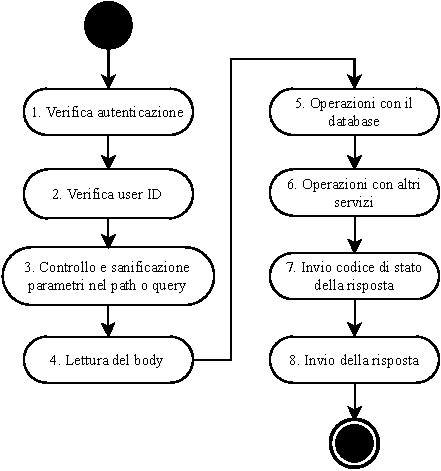
\includegraphics[width=0.7\textwidth]{assets/04/operazioni-api.pdf}
\caption{Passi operativi della gestione di una richiesta per una API.}
\label{fig:operazioni-api}
\end{figure}

L'implementazione di \texttt{GET /chats/\{chatid\}/messages/} viene mostrata come esempio nel listato di codice \ref{listing:impl_api}. Per compattezza il codice relativo alla gestione degli errori è stato nascosto tranne che nel primo caso. Infatti è interessante notare una peculiarità del linguaggio: Go non ha un sistema di eccezioni, la gestione degli errori è esplicita in modo simile al C. Scrivere codice in Go richiede perciò di gestire ogni caso di errore, e il linguaggio aiuta in ciò permettendo la restituzione di più valori da una funzione. A ogni percorso di errore viene stampato un messaggio di log e restituito un codice di errore al client.

Nelle ultime righe di codice è possibile notare come viene creata la risposta: la variabile \texttt{messages} consiste in una sequenza di messaggi e viene convertita in rappresentazione JSON. Tale rappresentazione viene scritta direttamente nel body della risposta, in automatico viene impostato il codice di stato \texttt{200}.

Oltre alla funzione mostrata, c'è parte di codice relativo alla costruzione dei parametri passati nella funzione, la verifica del token di autenticazione, che contiene anche l'user ID, e vario altro codice relativo al sistema in generale.

\begin{longlisting}
\begin{minted}{go}
func (rt *_router) getMessages(w http.ResponseWriter, r *http.Request, ps httprouter.Params, ctx reqcontext.RequestContext) {
	if ctx.UserID == uuid.Nil {
		ctx.Logger.Info("getChats: userid nil")
		w.WriteHeader(http.StatusBadRequest)
		return
	}

	chatid, err := strconv.ParseUint(ps.ByName("chatid"), 10, 64)
	if err != nil {
		// ...
	}

	var fromid uint64
	if rawFromid := r.URL.Query().Get("fromID"); rawFromid != "" {
		var err error
		if fromid, err = strconv.ParseUint(rawFromid, 10, 64); err != nil {
		    // ...
		}
	}

	if _, err = rt.DB.GetUsername(ctx.UserID); err != nil {
		// ...
	}

	messages, err := rt.DB.GetLatestMessages(chatid, fromid)
	if err != nil {
		// ...
	}

	w.Header().Set("content-type", "application/json")
	if err := json.NewEncoder(w).Encode(messages); err != nil {
		// ...
	}
}
\end{minted}
\caption{Implementazione di \texttt{GET /chats/\{chatid\}/messages/}.}
\label{listing:impl_api}
\end{longlisting}

\paragraph{Implementazione per package \texttt{database}} Nel codice mostrato in precedenza è possibile notare che durante la gestione vengono effettuate delle operazioni sul database tramite i metodi \texttt{GetUsername} e \texttt{GetLatestMessages}. Questi metodi contengono la logica per interagire con il database, principalmente la query SQL che viene eseguita, come mostrato nel listato di codice \ref{listing:impl_db} che implementa \texttt{GetLatestMessages}.

La query SQL è costruita in modo di mappare i nomi delle colonne con quelli della struttura \texttt{types.APIMessage}, perché, grazie alla riflessione (indicata anche come \textit{reflection}) di Go, è possibile effettuare una conversione automatica dai tipi del database con quelli della struttura. Il vantaggio di tale uso è la semplicità di scrittura del codice, a costo di una leggera penalità in prestazioni causate dalla riflessione.

\begin{longlisting}
\begin{minted}{go}
func (db *appdbimpl) GetLatestMessages(chatid uint64, fromid uint64) ([]types.APIMessage, error) {
	const (
		queryMessages = `
		SELECT message.id AS id,
			message.createdat AS createdat,
			user.name AS sentby,
			message.type AS type,
			IF(message.type = 'text', message.textcontent, "") AS text,
			IF(message.type = 'slider', message.intcontent, 0) AS slider,
			IF(message.type = 'image', message.textcontent, "") AS image
		FROM message JOIN user ON message.senderid = user.id
		WHERE (chatid = ?) AND (? = 0 OR message.id < ?)
		ORDER BY createdat DESC, id DESC
		LIMIT 25
		`
		queryMessage = `SELECT id FROM message WHERE id = ?`
	)

	// Controllo dell'esistenza di chatid e fromid...

	var latestMessages []types.APIMessage
	if err = db.c.Select(&latestMessages, queryMessages, chatid, fromid, fromid); err != nil {
		return nil, err
	}

	return latestMessages, nil
}
\end{minted}
\caption{Implementazione \texttt{GetLatestMessages}.}
\label{listing:impl_db}
\end{longlisting}

\section{Implementazione nel Worker}

Il Worker nella sostanza è una programma che lancia dei lavori periodici, anche chiamati \textit{task}. Sfrutta molto la concorrenza con le goroutine, infatti quello che fa è avviare dei timer, indipendenti l'uno dall'altro, a cui è associato un task. I timer ogni volta che scattano avviano il task in una nuova goroutine. Il funzionamento è schematizzato nella figura \ref{fig:ciclo_worker}. Sono due i task implementati per la funzionalità delle chat:

\begin{itemize}
\item \texttt{closeChats}: task eseguito in ogni minuto che si occupa di chiudere le chat che non sono state associate ad alcun terremoto entro un tempo arbitrario, per il momento deciso a 24 ore;
\item \texttt{matchChats}: task eseguito in ogni minuto che si occupa di assegnare un terremoto a una chat, in base alla posizione geografica e al tempo di creazione, confrontando gli ultimi terremoti con i dati delle chat.
\end{itemize}

\afterpage{\clearpage}

\begin{figure}[ht!]
\centering
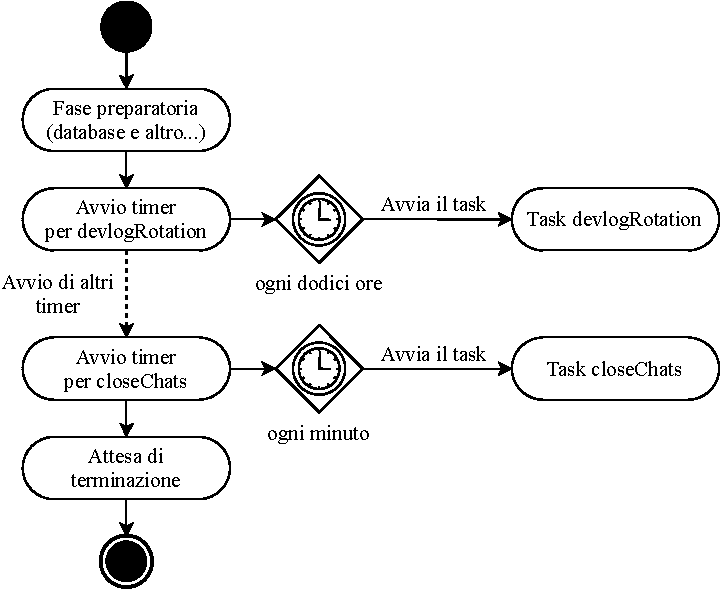
\includegraphics[width=0.85\textwidth]{assets/04/ciclo_vita_worker.pdf}
\caption{Ciclo di vita del Worker.}
\label{fig:ciclo_worker}
\end{figure}

Viene portato come esempio l'implementazione del task \texttt{closeChats} nel listato di codice \ref{listing:impl_worker}. In questo caso consiste soltanto di una query SQL di aggiornamento.

\begin{longlisting}
\begin{minted}{go}
func (w *_worker) closeChats() {
	const query = `
	UPDATE chat
	SET closed = TRUE
	WHERE closed = FALSE AND earthquakeid IS NULL AND createdat < NOW() - INTERVAL 24 HOUR
	`

	res, err := w.db.Exec(query)
	if err != nil {
		// ...
	}
	
	// Codice di log...
}
\end{minted}
\caption{Implementazione del task \texttt{closeChats} in Worker.}
\label{listing:impl_worker}
\end{longlisting}

\section{Test}

Durante l'implementazione delle API e dei task nel Worker sono state effettuate diverse prove manuali nell'ambiente di sviluppo locale. Dei vari tipi di test possibili, si sono preferiti quelli di integrazione per provare le API, verificando i risultati nel database o nelle risposte HTTP. In un secondo momento si è tentato di automatizzare in modo parziale i test tramite un programma scritto in Go che effettua le richieste e controlla la risposta per tutte le API. Il listato di codice \ref{listing:impl_test} mostra la funzione \texttt{TestPutUsername} che verifica i possibili codici di stato ritornati dall'API \texttt{PUT /me/username}. La funzione \texttt{testPutUsername} costruisce e invia la richiesta HTTP, poi verificare il codice di stato con quello passato come argomento.

La soluzione costruita non è risultata del tutto soddisfacente: per poter lanciare il programma di test è necessario configurare manualmente il servizio di autenticazione Keycloak, inoltre il database deve essere riportato allo stato originario dopo ogni esecuzione.

\begin{longlisting}
\begin{minted}{go}
func TestPutUsername(t *testing.T) {
	t.Run("200-OK", func(t *testing.T) {
		testPutUsername(t, "Giampiero", http.StatusOK)
	})
	t.Run("400-TOO-SHORT", func(t *testing.T) {
		testPutUsername(t, "Gi", http.StatusBadRequest)
	})
	t.Run("400-EMPTY-BODY", func(t *testing.T) {
		testPutUsername(t, "", http.StatusBadRequest)
	})
	t.Run("400-TOO-LONG", func(t *testing.T) {
		testPutUsername(t, "usernamemoltomoltomoltomoltolungo...", http.StatusBadRequest)
	})
}
\end{minted}
\caption{Esempio di test per \texttt{PUT /me/username}.}
\label{listing:impl_test}
\end{longlisting}

\chapter{Conclusione}
\label{ch:concl}

\section{Risultato ottenuto}

Partendo dai lavori di progettazione di Michele Spina, in questa relazione è stato descritto il lavoro che ha portato all'implementazione di una versione minimale ma funzionante, chiamata anche \textit{minimum viable product } (MVP). In questa versione sono state progettate, sviluppate e implementate le sole funzionalità necessarie per l'effettiva messa in produzione del sistema. L'obiettivo è quello di ottenere feedback da parte degli utenti per veicolare al meglio gli sviluppi futuri. Anche per questo motivo il sistema è stato progettato in modo da essere facilmente modificabile ed estensibile.

\section{Sviluppi futuri}

Sono molti gli spunti emersi durante il lavoro. Prima di tutto è però bene precisare che per poter mettere in produzione il sistema è necessario un ulteriore lavoro di adattamento delle API con i client e di progettazione delle rispettive interfacce utente. In questa sezione vengono tuttavia specificati punti di sviluppo futuro solo per il lato server e per la funzionalità in generale.

\paragraph{Algoritmo migliore per la creazione chat} Il punto critico dell'intero sistema è come il server determina la creazione di una chat in base a una richiesta ricevuta. Quando una chat viene creata per semplicità si associa la posizione geografica dell'utente che ha fatto la richiesta, ma tale associazione è approssimativa rispetto al terremoto. L'idea è quella di esplorare algoritmi più precisi e che reagiscano anche alle altre richieste di creazione, per esempio salvando in una lista le posizioni invece di salvare solo la prima. La raccolta di dati sulle posizioni geografiche è importante, perché influisce sulla generazione del nome della chat e sull'associazione con un terremoto.

\paragraph{Test più robusti} Attualmente la soluzione adottata per i test è fragile e richiede l'intervento umano, consuma perciò anche molto tempo. L'idea è quella di strutturare meglio i test, creando un ambiente automatizzato e riproducibile per l'esecuzione dei test di integrazione, e poi scrivere e documentare i test unitari per le parti di codice in Go. In aggiunta i test di carico possono tornare utili per identificare i punti deboli del sistema che lo possono rallentare.

\paragraph{Sistema delle notifiche} Nel sistema costruito è previsto l'invio delle notifiche basandosi sulle sottoscrizioni degli utenti, ma manca il sistema sottostante per l'invio effettivo di tali notifiche. Poiché tale sistema dipende strettamente dai sistemi operativi Android e iOS, l'idea è di appoggiarsi al servizio esterno Firebase Cloud Messaging di Google, che permette di inviare notifiche push.

\paragraph{Istanza Nominatim di SeismoCloud} Per il momento nella generazione del nome di una chat e nell'associazione a un terremoto viene utilizzata l'istanza pubblica di Nominatime offerta da OpenStreetMap. Tale istanza impone dei limiti d'uso che sono adatti a delle interrogazioni sporadiche e non a un uso intensivo come fa SeismoCloud. Per tale ragione è necessario costruire un'istanza interna e personalizzata per gli scopi della funzionalità.



\chapter{Ringraziamenti}
\label{ch:ringr}

In questi quattro anni trascorsi sono state molte le persone che hanno influito su di me e che mi hanno aiutato. Sono certo che molte di loro neanche ne sono consapevoli, ma io le ricorderò nel mio cuore.

Devo ringraziare il mio relatore il Prof. Emanuele Panizzi, che mi ha permesso di partecipare a un lavoro innovativo e stimolante, in cui mi sono messo in gioco e ho espresso le mie qualità sotto la sua guida. Non posso non ringraziare il dottorando Enrico Bassetti, per tutte le volte che mi ha aiutato nel proseguire il lavoro e per le interminabili discussioni sul mondo dell'informatica dai risvolti mai banali.
 
L'ultimo anno e mezzo è stato un periodo difficile, per cui devo ringraziare tutti coloro che mi sono stati accanto, sia fisicamente sia a distanza, senza di loro non avrei retto. Tra tutti devo porre l'attenzione sui miei genitori, che sono stati fondamentali sostenendomi in tutti i modi possibili.

Sono soddisfatto del risultato raggiunto dopo quattro anni di fatiche, tuttavia lo vedo come un punto di partenza che di arrivo, verso qualcosa di molto più grande e di mio che posso costruire e modellare seguendo i miei sogni.



\backmatter


\addcontentsline{toc}{chapter}{\protect\textbf{Elenco delle figure, tabelle e codici sorgente}}
% Forza l'elenco delle figure, delle tabelle e dei codici sorgente uno dietro l'altro, invece di iniziare sempre su recto.
{\listoffigures \let\cleardoublepage\null \listoftables \let\cleardoublepage\null \listoflistings}

\cleardoublepage

\printbibliography[heading=bibintoc]

\end{document}